% !TeX root = ../latex-talk.tex

\title{如何使用 beamer 制作学术报告幻灯片}
\subtitle{上海交通大学图书馆专题培训讲座}
\author{李子龙}
\institute[SJTU Linux User Group]{上海交通大学 Linux 用户组}
\date{2022 年 5 月}
\subject{LaTeX, 幻灯片制作, SJTUBeamer}
\maketitle

\providecommand{\TikZ}{Ti\textit{k}Z}
\providecommand{\pgf}{\textsc{pgf}}

\begin{frame}{关于}
  \begin{columns}[c]
  \begin{column}{.7\textwidth}
    \begin{block}{如何使用 beamer 制作学术报告幻灯片}
    \alert{\url{https://github.com/sjtug/sjtulib-latex-talk}}
    
    \begin{flushleft}
      \small 介绍 \LaTeX{} 幻灯片模板 \textsc{SJTUBeamer} 的使用方法,以及 \LaTeX{} 图形绘制的简明方法,帮助学生制作出像模像样的学术幻灯片。
    \end{flushleft}

    \begin{tabular*}{0.8\linewidth}{@{\extracolsep{\fill}}lll@{}}
      \scriptsize 最后更新 & \scriptsize 幻灯片下载 & \scriptsize 许可证 \\
      \today & Overleaf \link{https://www.overleaf.com/read/fvwxzvcxhcwd} & \href{https://creativecommons.org/licenses/by-sa/4.0/}{\faCreativeCommons\,\faCreativeCommonsBy\,\faCreativeCommonsSa} \\ 
    \end{tabular*}
    \end{block}
    \vspace{0.2cm}
  \end{column}
  \begin{column}{.3\textwidth}
    \qrcode[hyperlink, height=4cm]{https://www.overleaf.com/read/fvwxzvcxhcwd}
  \end{column}
  \end{columns}
\end{frame}

\begin{frame}
  \frametitle{讲稿主要参考}
  \begin{bibliolist}{00}
    \onlineitem 吕荐瑞.
    \newblock \LaTeX{} 文档排版教程[EB/OL].
    \newblock 2018. \url{https://lvjr.bitbucket.io/tutorial/learn-latex.pdf}
    
    \onlineitem \LaTeX{} 工作室.
    \newblock \TikZ{} \& \pgf{} 手册 (3.1.5b) 笔记[EB/OL].
    \newblock 2020. \url{https://www.latexstudio.net/archives/51804.html}
    
    \onlineitem \textsc{Hansimov}. 
    \newblock 如何加速 \LaTeX{} 编译[EB/OL].
  \newblock 2019. \url{https://zhuanlan.zhihu.com/p/55043560}
  \end{bibliolist}
\end{frame}

% !TeX root = ../../latex-talk.tex

\part{SJTUBeamer}

\begin{frame}
  \frametitle{简介}
  \begin{columns}
    \begin{column}{0.6\textwidth}
      \begin{itemize}
        \item 最早由谌翔于 2021 年 4 月发布
        \item 2021 年 5 月起由 SJTUG 接手,发布 1.0 版
        \item 2021 年 9 月李子龙重构了整个宏包的代码,升级版本号为 2.0
        \item 最新版:\SJTUBeamerVersion{} (\SJTUBeamerDate)
        \item 支持三种基本样式与扩展样式的幻灯片模板
        \item 支持镜像站克隆 \link{https://mirror.sjtu.edu.cn/git/SJTUBeamer.git/},支持使用任一引擎编译
      \end{itemize}
    \end{column}
    \begin{column}{0.4\textwidth}
      \begin{exampleblock}{}
        \begin{minipage}[c]{1cm}
          
\includegraphics[width=0.8cm]{support/examples/pics/sjtug.pdf}
        \end{minipage}
        \begin{minipage}[c]{4cm}
          \href{https://github.com/sjtug}{sjtug}/\href{https://github.com/sjtug/SJTUBeamer}{SJTUBeamer}
        \end{minipage}
      \end{exampleblock}
      \vspace{-8pt}
      \begin{block}{}
        \scriptsize
        上海交通大学 Beamer 模版 | Beamer template for Shanghai Jiao Tong University
      \end{block}
      \vspace{-8pt}
      \begin{alertblock}{}
        \scriptsize
        \begin{tabular}{cl}
          \faStar       & 357 \\
          \faEye        & 7   \\
          \faCodeBranch & 29  \\
        \end{tabular}
      \end{alertblock}
    \end{column}
  \end{columns}
\end{frame}

\begin{frame}
  \frametitle{\only<1>{为什么使用 beamer 制作幻灯片?}\only<2>{当然也有新兴替代物}}
  \begin{columns}[t]

    \only<2>{
      \begin{column}{0.25\textwidth}
        \begin{block}{\faMarkdown{} 代码翻译}
          \begin{itemize}
            \item[\faVuejs{}] Slidev \link{https://cn.sli.dev/}
            \item[\faJsSquare{}] Marp \link{https://marp.app/}
            \item[\faJs{}] AutoBeamer \link{https://github.com/LogCreative/AutoBeamer}
          \end{itemize}
        \end{block}
        \note[item]<2>{\textbf{Markdown} 当然也有新兴替代物,比如可以从 Markdown 代码转换为幻灯片的一些软件。基于 Vue 的 Slidev 可以快速地输出灵活布局的幻灯片,基于 TypeScript 的 Marp 可以作为 VS Code 的插件来实时预览 Markdown 幻灯片,还有我制作的转换 Markdown 文档为 beamer 代码的 AutoBeamer 也欢迎大家的试用。}
      \end{column}
    }

    \begin{column}{0.25\textwidth}
      \begin{block}{\LaTeX{} SJTUBeamer}
        \begin{itemize}
          \item[\faPlus] \LaTeX{} 原生
          \item[\faPlus] 规范的格式
          \item[\faMinus] 美术功能麻烦
        \end{itemize}
      \end{block}
      \note[item]<1>{\textbf{Beamer} 是 \LaTeX{} 原生的幻灯片类,可以输入专业的公式,其编程式的方法会促使用户规整幻灯片的布局,更为容易地产生正式而不失优雅的幻灯片。我们使用 \LaTeX{} 主要也是为了符合规范,对于很多不擅长排版的小伙伴有个这样的工具自动美化自己的作品是一件非常方便的事情。

        当然缺点也是存在的,就是美术功能的实现较为复杂,以及一些多媒体的支持可能需要使用链接的形式。}
    \end{column}

    \only<2>{
      \begin{column}{0.25\textwidth}
        \begin{exampleblock}{\faApple{} Keynote}
          \begin{itemize}
            \item[\faPlus] 友好的界面
            \item[\faPlus] 精致的动画
            \item[\faMinus] 缺少进阶功能
          \end{itemize}
        \end{exampleblock}
        \note[item]<2>{\textbf{Keynote} 是苹果独占的幻灯片软件,相比于 PowerPoint 有了更加用户友好的界面,辅以一些精致的动画,可以较快地做出“果味”幻灯片。

          当然简单也会带来进阶功能的缺失,缺乏插件体系的支持,能做出的东西相比于 PowerPoint 少了不少。}
      \end{column}
    }

    \begin{column}{0.25\textwidth}
      \begin{exampleblock}{\faFilePowerpoint{} PowerPoint}
        \begin{itemize}
          \item[\faPlus] 灵活的插件
          \item[\faPlus] 强大的动画
          \item[\faMinus] 布局不够规整
        \end{itemize}
      \end{exampleblock}
      \note[item]<1>{\textbf{PowerPoint} 我们在前半部分的讲座中看到了 PowerPoint 制作幻灯片的强大之处,可见即可得,辅以强大的动画功能,并可以使用灵活的插件提高效率。

        当然灵活性也会让用户在布局上更加随意一些,并在这样一些细节上让整个演讲稿看起来慢慢地变得没有那么正式。当然你也可以只使用大纲视图编写幻灯片,来规整自己的布局。}
    \end{column}
  \end{columns}
\end{frame}

\begin{frame}
  \frametitle{浅学手册}

  \only<1>{
    \begin{columns}
      \begin{column}{0.7\textwidth}
        前往 SJTUBeamer 的发布页 \link{https://github.com/sjtug/SJTUBeamer/releases} 可以得到一个干净的 \pkg{sjtubeamer-ctan.zip},用于将该 SJTUBeamer 安装到本地目录。以及一些其他文档的下载。当然你也可以在 SJTUG 镜像站 \link{https://mirror.sjtu.edu.cn/} 上下载 SJTUBeamer 的这些 Assets。

        \begin{exampleblock}{\faGit* 从镜像站克隆最新版}
          \ttfamily\footnotesize
          git clone https://mirror.sjtu.edu.cn/git/SJTUBeamer.git/
        \end{exampleblock}
      \end{column}
      \begin{column}{0.3\textwidth}
        \fzerobox{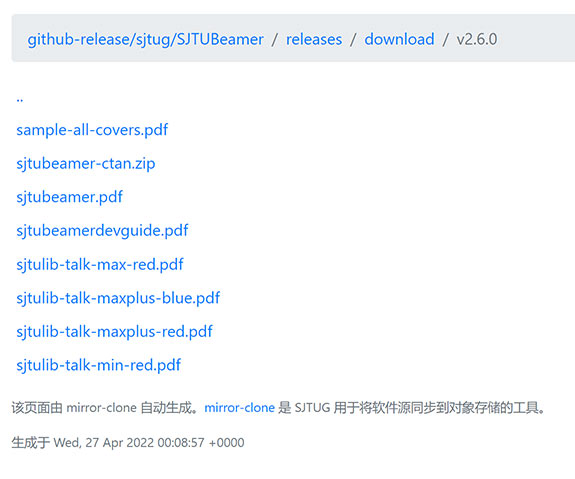
\includegraphics[width=\linewidth]{support/images/mirrorclone.jpg}}
      \end{column}
    \end{columns}
    \note[item]{GitHub 上克隆的是开发版(社区版),Release 得到的是稳定版,虽然开发版比稳定版稳定,但是稳定版在镜像站的加持下下载会更快一些。}
    \note[item]{进入镜像站页面后,点击 github/SJTUBeamer(点击 git/SJTUBeamer.git 会有 BUG)。}
  }

  \only<2>{
    \begin{columns}
      \begin{column}{0.7\textwidth}
        《SJTUBeamer 使用手册》\link{https://github.com/sjtug/SJTUBeamer/releases/download/v\SJTUBeamerVersion{}/sjtubeamer.pdf} 给出了大量的示例,用于快速上手 SJTUBeamer 的基本使用方法。推荐大家从一个干净的文档一步步码出来这些例子,或者遇到问题先按手册查询。本讲座仅做概览。

        \note{这些例子含有 beamer 文档类的基础用法,一步步地完成可以较快地学会这些知识。}

        \begin{exampleblock}{\faTerminal{} 从源码编译文档}
          \ttfamily\footnotesize
          cd src\\
          l3build doc
        \end{exampleblock}
      \end{column}
      \begin{column}{0.3\textwidth}
        \fzerobox{
\includegraphics[width=\linewidth]{support/images/sjtubeamerfirst.jpg}}
      \end{column}
    \end{columns}
  }

  \only<3>{
    \begin{columns}
      \begin{column}{0.7\textwidth}
        \textit{Development Guide of SJTUBeamer} \link{https://github.com/sjtug/SJTUBeamer/releases/download/v\SJTUBeamerVersion{}/sjtubeamerdevguide.pdf} 对于想要了解 SJTUBeamer 框架与原理的人会比较有用,感兴趣的可以通过阅读该手册尝试对代码更改提 PR 或贡献插件 \link{https://github.com/sjtug/SJTUBeamer/issues/81}。本讲座不会涉及这一部分。
        \begin{exampleblock}{\faTerminal{} 代码同步}
          \ttfamily\footnotesize
          cd src\\
          \textcolor{gray}{\# 将 Doc\TeX{} 解包为 sty 文件并移至根目录} \\
          l3build check
        \end{exampleblock}
      \end{column}
      \begin{column}{0.3\textwidth}
        \fzerobox{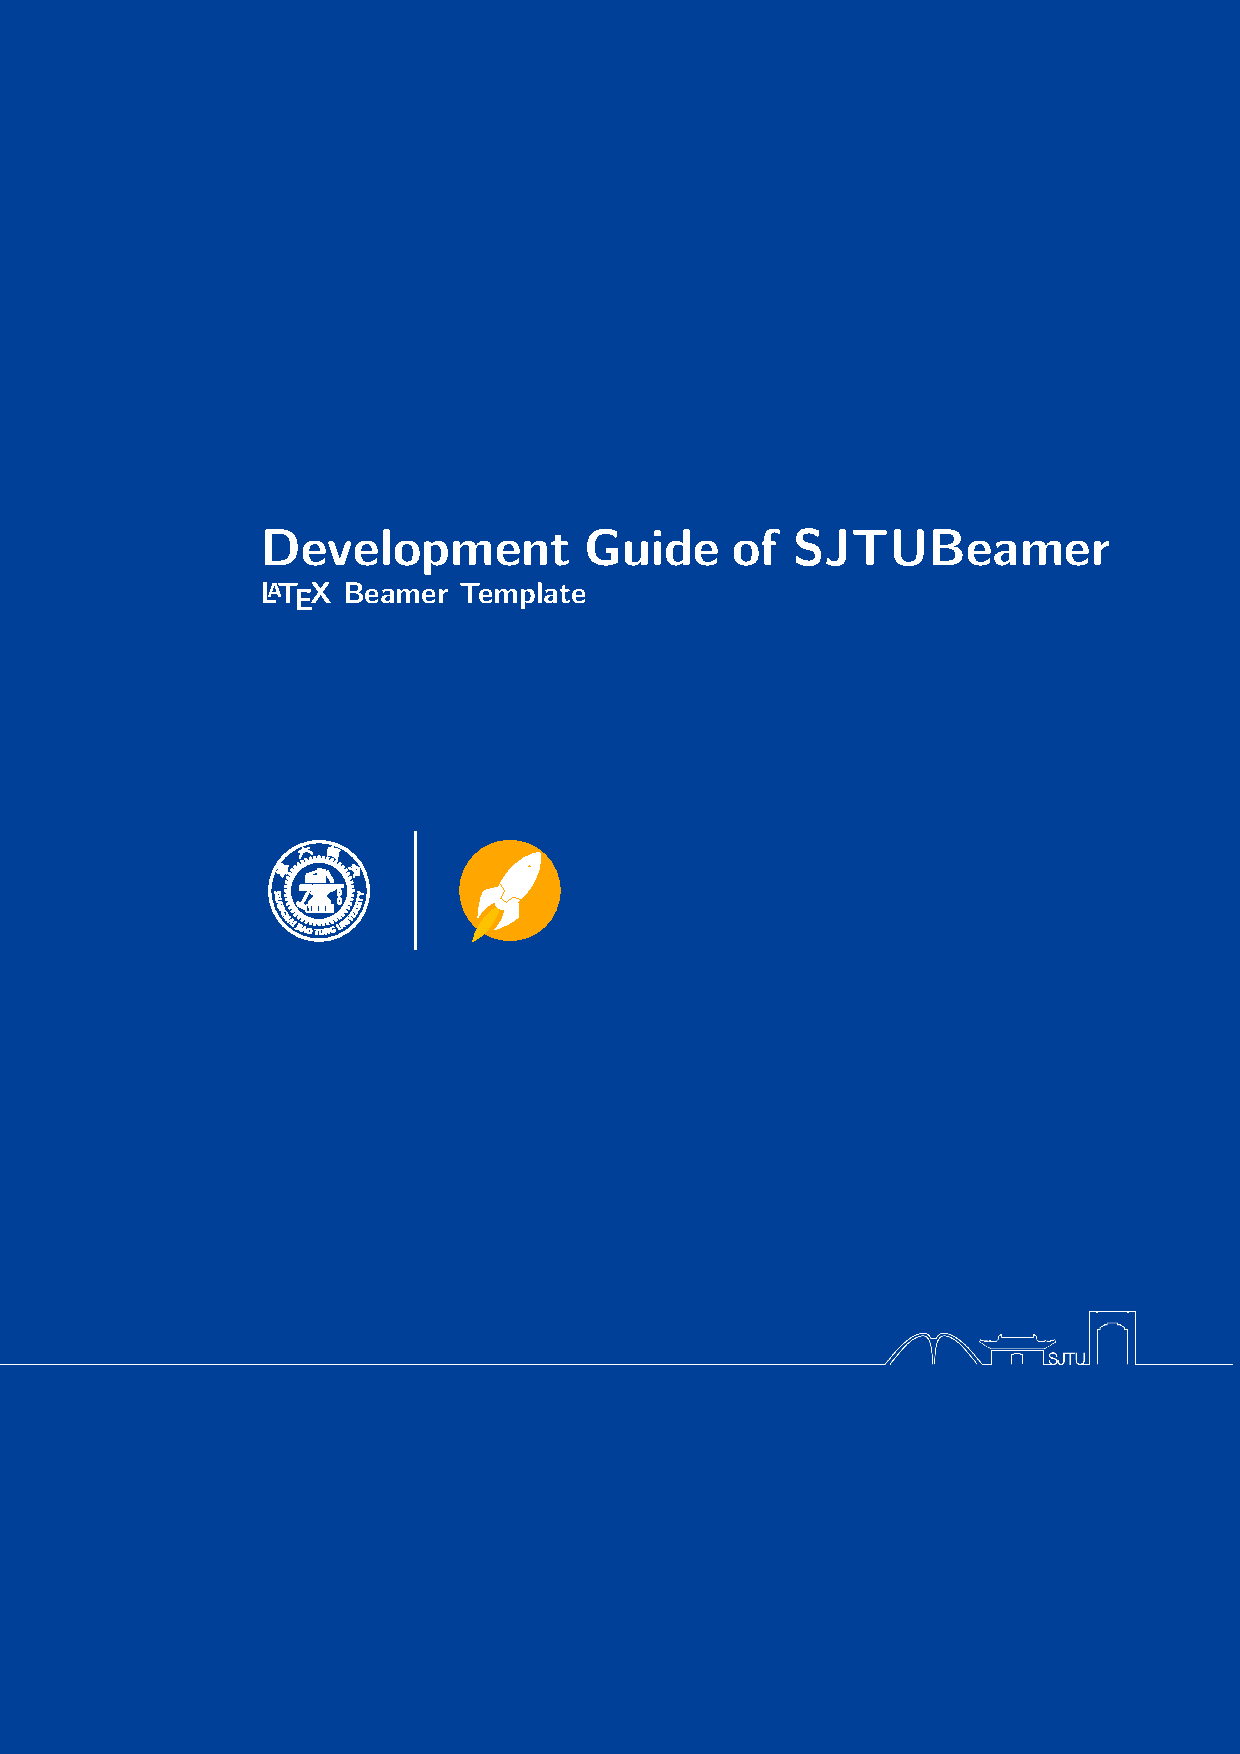
\includegraphics[width=\linewidth]{support/images/sjtubeamerdevguidefirst.pdf}}
      \end{column}
    \end{columns}
    \note{用英文写开发手册实际上是因为国内做 beamer 的比较少。sad。}
  }

\end{frame}

\begin{frame}[fragile]
  \frametitle{文档类设置}

  \only<1>{
    为文档类设置 \opt{aspectratio} 选项可以更改幻灯片的长宽比。其他通用选项详见 \textit{The Beamer Class -- User Guide} \link{https://mirrors.sjtug.sjtu.edu.cn/CTAN/macros/latex/contrib/beamer/doc/beameruserguide.pdf}。帧环境 \env{frame} 详见第 \ref{frame} 页。
    \note{有些教室可能还在用 4:3 比例(不调整默认是 4:3 比例),在 beamer 里调整比例要比 PowerPoint 里要方便的多,因为内容与格式分离了,不会导致比例失调的情况。}
  }

  \only<2>{
    SJTUBeamer 依赖于 \cls{ctexbeamer} 文档类,相关字体设置详见《\CTeX{} 宏集手册》\link{https://mirrors.sjtug.sjtu.edu.cn/CTAN/language/chinese/ctex/ctex.pdf}。如果编写英文幻灯片,请直接使用 \cls{beamer} 文档类。
    \note{\opt{fontset} 可以被指定为诸如 \opt{ubuntu}, \opt{adobe}, \opt{founder} 等,注意 SJTUThesis 中只能使用 \opt{cjk-font} 调整,暂时没有为 SJTUBeamer 设定单独字体样式的想法,毕竟幻灯片跟论文还是不太相同的。当然如果以后有什么“交大字体”啦,我们可以考虑适配一下。}
  }

  \begin{columns}
    \begin{column}{0.62\textwidth}
      \begin{codeblock}[]{\only<1>{更改长宽比}\only<2>{更改字体}}
|\highlightline|\documentclass[|\only<1>{aspectratio=169}\only<2>{fontset=fandol}|]{ctexbeamer}
\usetheme{sjtubeamer}
\begin{document}
  \begin{frame}
    \frametitle{|\phantom{}|欢迎}
    |\phantom{}|你好,SJTUBeamer|\phantom{}|!
|\phantom{}|  \end{frame}
|\phantom{}|\end{document}
      \end{codeblock}
    \end{column}
    \begin{column}{0.38\textwidth}
      \begin{center}
        \includebeamerlarge{support/beamer/welcome.pdf}
      \end{center}
    \end{column}
  \end{columns}
\end{frame}

\begin{frame}[fragile]
  \frametitle{切换设计}
  \begin{columns}
    \begin{column}{0.6\textwidth}

      \only<1>{
        为了使用 SJTUBeamer,需要在根目录中创建一个文件,并添加 \cmd{usetheme\{sjtubeamer\}}。你可以添加用逗号分隔的选项切换不同的设计样式。
        \note{使用 \opt{maxplus}, \opt{max}, \opt{min} 切换不同的封面样式(包含节次页)。使用 \opt{red}, \opt{blue} 来切换主色调。使用 \opt{dark} 和 \opt{light} 来切换不同的亮度主题。}
      }

      \only<2>{
        还可以适配 \cls{beamer} 自带的外样式,可以通过 \opt{topright} 或 \opt{bottomright} 选项切换徽标位置。
        \note{
          使用外样式关键字切换页面布局,使用 \opt{topright} 和 \opt{bottomright} 切换徽标的位置。
        
          sidebar 外样式略有一些 BUG,就是封面页会有文字偏移,感兴趣地可以考虑修正一下,暂时没有找到太好的通用方法,这种情况下可以考虑不使用标题页或只使用 maxplus 版本。冷知识,10 年前也有学长做了个 \href{https://github.com/X-Wei/aBeamerTemplate4SJTU}{SJTU Beamer 模板}发布于水源 BBS,使用的就是 sidebar 外样式。
          
          别小看这两页,SJTUBeamer 很多代码都放在这两页上了,这两页已经可以组合出 $3\times 2\times 2\times 9\times 2=216$ 种可能了(忽略徽标位置的话正好 108 种)。每次展示都用同一种样式显得比较单调,适当的时候可以改改选项试试这些样式。}
      }

      \begin{codeblock}[]{}
\documentclass{ctexbeamer}
|\highlightline|\usetheme[|\only<1>{maxplus,blue,light}\only<2>{default,topright}|]{sjtubeamer}
\begin{document}
  \title{|\phantom{}|使用 Beamer 制作学术报告幻灯片}
  \subtitle{|\phantom{}|上海交通大学图书馆专题培训讲座}
  \author{|\phantom{}|李子龙}
  \institute[SJTUG]{SJTU Linux User Group}
  \date{2022 年 5 月}
|\highlightline<1>|  \maketitle
|\highlightline<1>|  \part{|\phantom{}|介绍}
|\highlightline<1>|  \makebottom
|\phantom{}|\end{document}
      \end{codeblock}
    \end{column}
    \begin{column}{0.4\textwidth}
      \only<1>{
        \begin{figure}
          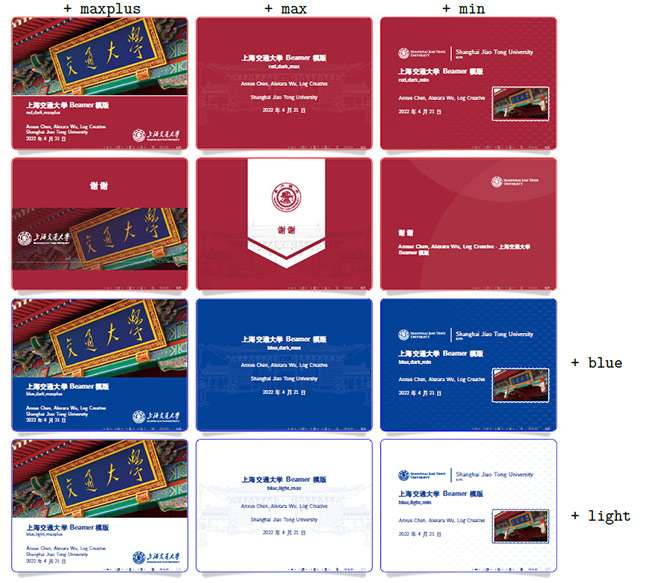
\includegraphics[width=\linewidth]{support/images/sjtubeamercover.jpg}
          \caption{封面样式}
        \end{figure}
      }
      \only<2>{
        \begin{figure}
          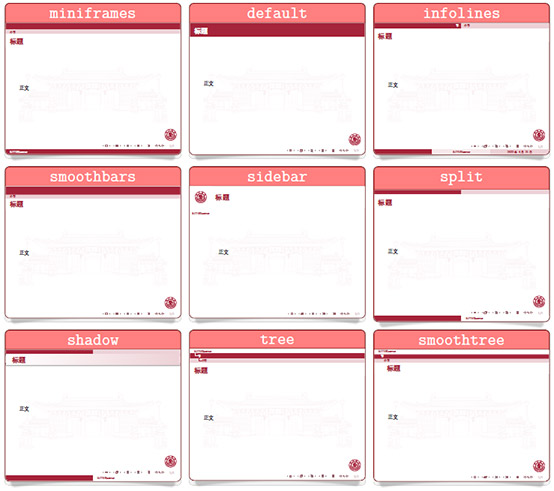
\includegraphics[width=\linewidth]{support/images/sjtubeamerouter.jpg}
          \caption{外样式}
        \end{figure}
      }
    \end{column}
  \end{columns}
\end{frame}

\begin{frame}[fragile]
  \frametitle{目录}
  \cmd{tableofcontents} 命令在 \cls{beamer} 中可以添加参数以更改要展示的节次标题。\opt{hideallsubsections} 参数用于不排印小节标题。
  \begin{columns}
    \begin{column}{0.6\textwidth}
      
      \begin{codeblock}[]{目录页}
|\phantom{}|\documentclass{ctexbeamer}
\usetheme{sjtubeamer}
\begin{document}
  \begin{frame}
    \frametitle{|\phantom{}|目录}
|\highlightline|    \tableofcontents[hideallsubsections]
  |\phantom{}|\end{frame}
|\phantom{}|\end{document}
      \end{codeblock}
      
    \end{column}
    \begin{column}{0.4\textwidth}
      \centering
      \includebeamerlarge[1]{support/beamer/toc.pdf}
    \end{column}
  \end{columns}
\end{frame}

\begin{frame}[fragile]
  \frametitle{目录}
  \only<1>{
    \cmd{AtBeginSection} 用于向每节开始添加内容。
  }

  \only<2>{
    最常见的做法是添加当前节的高亮目录,添加 \opt{currentsection} 参数高亮该节。
  }

  \begin{columns}
    \begin{column}{0.6\textwidth}
      
      \begin{codeblock}[]{节目录}
|\phantom{}|\documentclass{ctexbeamer}
\usetheme{sjtubeamer}
|\highlightline<1>|\AtBeginSection[]{
  \begin{frame}
|\highlightline<2>|    \tableofcontents[currentsection, hideallsubsections]
  |\phantom{}|\end{frame}
|\highlightline<1>|}
\begin{document}
  \section{|\phantom{}|第一节}
|\phantom{}|\end{document}
      \end{codeblock}
      
    \end{column}
    \begin{column}{0.4\textwidth}
      \centering
      \includebeamerlarge[2]{support/beamer/toc.pdf}
    \end{column}
  \end{columns}
\end{frame}

\begin{frame}[fragile]
  \frametitle{目录}
  也可以通过 \cmd{sectionpage} 添加节页,在 SJTUBeamer 里最好在帧上添加 \opt{plain} 参数,以隐藏导航栏。

  \begin{columns}
    \begin{column}{0.6\textwidth}
      
      \begin{codeblock}[]{节页}
|\phantom{}|\documentclass{ctexbeamer}
\usetheme{sjtubeamer}
\AtBeginSection[]{
|\highlightline|  \begin{frame}[plain]
|\highlightline|    \sectionpage
  |\phantom{}|\end{frame}
}
\begin{document}
  \section{|\phantom{}|第一节}
|\phantom{}|\end{document}
      \end{codeblock}
      
    \end{column}
    \begin{column}{0.4\textwidth}
      \centering
      \includebeamerlarge[5]{support/beamer/toc.pdf}
    \end{column}
  \end{columns}
\end{frame}

\begin{frame}
  \frametitle{符合交大视觉形象识别系统}

  \begin{table}
    \caption{上海交通大学视觉形象识别系统规范(节选)}
    \vspace*{-5pt}
    \begin{stampbox}
      \footnotesize
      \begin{tabular}{llll}
        \alert{编号}                                                   & \alert{说明}                   & \alert{编号}                                                   & \alert{说明}     \\
        \href{https://vi.sjtu.edu.cn/index.php/articles/base/1}{A1-06} & 校徽需 $\frac{1}{5}h$ 安全空间 & \href{https://vi.sjtu.edu.cn/index.php/articles/base/5}{A5-03} & 辅助图形使用规范 \\
        \href{https://vi.sjtu.edu.cn/index.php/articles/base/3}{A3-01} & 标准色规范(含色阶)           & \href{https://vi.sjtu.edu.cn/index.php/articles/base/5}{A5-05} & 辅助图形底纹制作 \\
        \href{https://vi.sjtu.edu.cn/index.php/articles/base/3}{A3-02} & 辅助色彩规范(含色阶)         & \href{https://vi.sjtu.edu.cn/index.php/articles/app/7}{B1-01}  & 名片             \\
        \href{https://vi.sjtu.edu.cn/index.php/articles/base/3}{A3-05} & 品牌专用色彩搭配表             & \href{https://vi.sjtu.edu.cn/index.php/articles/app/7}{B1-20}  & 文件封套         \\
        \href{https://vi.sjtu.edu.cn/index.php/articles/base/4}{A4-08} & 二级机构中英文名称横式组合     & \href{https://vi.sjtu.edu.cn/index.php/articles/app/8}{B2-02}  & PPT 模板         \\
      \end{tabular}
    \end{stampbox}
  \end{table}

  正如 SJTUThesis 需要依照学位论文规范一样,SJTUBeamer 借助于 \TikZ{} 实现了《上海交通大学视觉形象识别系统》\link{https://vi.sjtu.edu.cn/} 的绝大部分规范\footnote{使用规范所规定的用品需要遵守相关许可条例 \link{https://vi.sjtu.edu.cn/index.php/articles/bulletin/16}。}。

  \note[item]{我相信小米的二百万 logo 更改让大家意识到了视觉形象识别系统的存在。交大在 2016 年的时候颁布了自己的视觉形象识别系统,并配套了对应的 PPT 模板。}

  \note[item]{许可条例第十三条规定:“校属各单位及个人可以自行或委托其他单位制作《手册》中有明确范例的物品,须严格遵照《手册》的要求,不得自行改动”,\textsc{SJTUBeamer} 也就需要依照该规范制作产物。}
\end{frame}

\begin{frame}
  \frametitle{SJTU VI 对应的特殊方法}

  \begin{columns}
    \begin{column}{0.7\textwidth}

      \stamptext[sjtuRedPrimary]{注} \cmd{stamptext} 用于创建一个印记形状文本框。

      \begin{stampbox}[sjtuRedPrimary]
        \env{stampbox} 环境用于创建一个印记盒子。
      \end{stampbox}

      \cmd{stamparray} 用于在 \env{tikzpicture} 环境(第 \ref{tikz} 页)中创建印记矩阵图案。\textcolor{structure}{$\blacktriangleright$}
    \end{column}
    \begin{column}{0.3\textwidth}
      \begin{figure}
        \centering
        \begin{tikzpicture}
          \setbeamercolor{palette primary}{bg=sjtuRedPrimary,fg=white}
          \stamparray{16pt}{(0,0)}{(4,3)}
        \end{tikzpicture}
        \caption{印记矩阵}
      \end{figure}
    \end{column}
  \end{columns}

  \note{SJTU 视觉形象识别系统规定的一些图案,采用 \TikZ{} 代码的方式绘制出来。}
\end{frame}

\begin{frame}[fragile]
  \frametitle{SJTUThesis 对应的特殊方法}
  \begin{columns}
    \begin{column}{0.55\textwidth}
      \env{codeblock} 环境用于创建代码抄录盒子。与 SJTUThesis 略有不同的是,它需要一个强制参数指定标题,并且注意在所在帧上添加 \opt{fragile} 选项。
    \end{column}
    \begin{column}{0.45\textwidth}
      \begin{codeblock}{代码盒子}
|\textbackslash{}begin\{codeblock\}|[language=python]{Python 代码}
|\phantom{}|print("Hello, world!")
|\textbackslash{}end\{codeblock\}|
      \end{codeblock}
    \end{column}
  \end{columns}

  \note[item]{当然你可以将 \env{codeblock} 环境的强制参数留空,但要保留大括号。这样就不会产生代码块的标题。}

  \begin{columns}
    \begin{column}{0.55\textwidth}
      \env{bibliolist} 环境用于手动创建引用文献列表。可以直接使用 SJTUThesis 的 \cmd{item} 式创建条目,也可以使用 \cmd{articleitem}, \cmd{bookitem}, \cmd{onlineitem} 配合 \cmd{newblock} 创建不同图标的条目。
    \end{column}
    \begin{column}{0.45\textwidth}
      \begin{bibliolist}{00}
        \onlineitem SJTUG.
        \newblock SJTUBeamer 使用手册[EB/OL].
        \newblock 2022. \url{https://github.com/sjtug/SJTUBeamer}
      \end{bibliolist}
    \end{column}
  \end{columns}

  \note[item]{\env{bibliolist} 的环境定义与 SJTUThesis 相同,但是对 \cls{beamer} 有了特殊的优化。}

\end{frame}

\begin{frame}
  \frametitle{SJTUBeamer 的其他附加方法}
  \highlight[sjtuBluePrimary]{高亮} \cmd{highlight} 用于产生高亮效果。
  
  \paragraph{段落} \cmd{paragraph} 在 \cls{beamer} 中原本是无效的。

  \vspace*{0.25em}

  \cmd{makebottom} 用于创建底页,\cls{beamer} 中只有 \cmd{maketitle}。

  \vspace*{1em}

  如果你需要迁移幻灯片至其他样式,可以尝试通过 \cmd{usetheme} 加载该存储库中的 \pkg{nosjtubeamer} 样式。\sout{或者是直接改个徽标}
\end{frame}

\begin{frame}[fragile]
  \frametitle{欢迎贡献主题}
  SJTUBeamer 设计了一套简单的接口,用于将幻灯片修改成你的主题!使用 \cmd{usesjtutheme} 调用社区版 \pkg{contrib} 文件夹内的插件 \link{https://github.com/sjtug/SJTUBeamer/issues/81},可以阅读对应插件附带的文档源码了解如何使用该插件。
  
  \begin{columns}
    \begin{column}{0.55\textwidth}
      \begin{codeblock}{使用子主题}
\documentclass{ctexbeamer}
\usetheme[my]{sjtubeamer}
|\highlightline|\usesjtutheme{sjtug}
\begin{document}
  \begin{frame}
    |\phantom{}|使用 SJTUG 子主题。
|\phantom{}|  \end{frame}
|\phantom{}|\end{document}
      \end{codeblock}
    \end{column}
    \begin{column}{0.45\textwidth}
      \begin{figure}
        \centering
        \includebeamerlarge{support/beamer/sjtug.pdf}
        \caption{SJTUG 子主题}
      \end{figure}
    \end{column}
  \end{columns}

  \note{有的插件并不需要向 sjtubeamer 设定 my 选项。下面来了解一下 \cls{beamer} 的基础模型,因为我觉得这些部分可能要比前面这些设定参数要难一点,所以放在了偏后的位置。以及 SJTUBeamer 对下面的内容优化程度可能还稍显不足。}
  \note{展示几个自建主题。}
  
\end{frame}

\begin{shadedsection}

\section{是什么}

\begin{frame}
  \frametitle{slides}

  \cls{slides} 是为 20 世纪 80 年代中期物理投影片开发的文档类。

  \begin{columns}
    \begin{column}{0.33\textwidth}
      \begin{figure}
        \centering
        \begin{stampbox}[sjtuRedPrimary]
          \scriptsize
          
\includegraphics[width=0.88\linewidth]{support/images/slides.jpg}
        \end{stampbox}
        \caption{幻灯影片}
      \end{figure}
    \end{column}
    \begin{column}{0.33\textwidth}
      \begin{figure}
        \centering
        \begin{stampbox}[sjtuRedPrimary]
          \scriptsize
          
\includegraphics[width=0.88\linewidth]{support/images/screen.jpg}
        \end{stampbox}
        \caption{准备荧幕}
      \end{figure}
    \end{column}
    \begin{column}{0.33\textwidth}
      \begin{figure}
        \centering
        \begin{stampbox}[sjtuRedPrimary]
          \scriptsize
          
\includegraphics[width=0.88\linewidth]{support/images/project.jpg}
        \end{stampbox}
        \caption{投影放映}
      \end{figure}
    \end{column}
  \end{columns}
  \footnotetext{图像由 nickelodeon 持有版权。} % Overleaf 版本将会将图像设为 draft
  \note{我拿海绵宝宝举例说明,首先准备好一卷幻灯影片,放入幻灯机后准备个荧幕,然后按下按钮切换不同的幻灯片,如果是以前的话,你还可以专门找个助手帮你切片,然后你示意一下去切片。}
\end{frame}

\begin{frame}
  \frametitle{beamer}

  \cls{beamer} 是含有一些 PDF 交互式演示功能的文档类。

  \begin{figure}
    \centering
    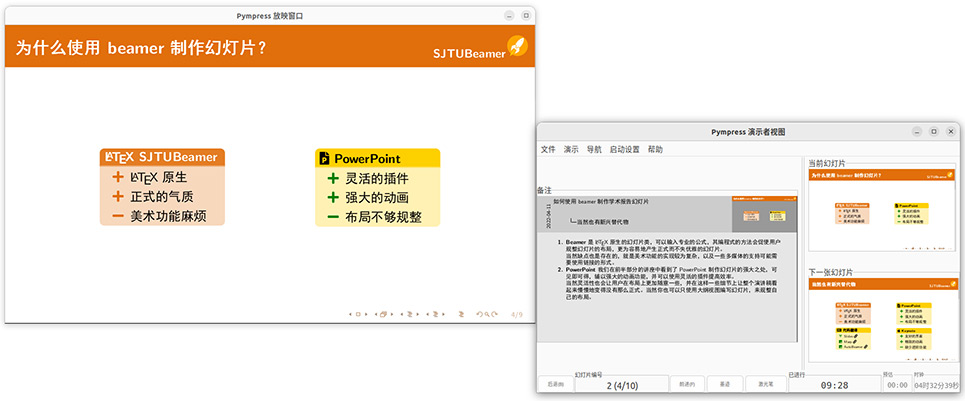
\includegraphics[width=0.7\linewidth]{support/images/pympress.jpg}
    \caption{Pympress 阅读器\footnote{需要使用 \cmd{note} 添加笔记,并在导言区添加 \cmd{setbeameroption\{notes on second screen\}} 以启用第二屏功能。} \link{https://github.com/Cimbali/pympress}}
    \note[item]{使用 Pympress 阅读器以最大化 beamer 的交互功能(左侧为放映窗口,右侧为演示者视图),并使用类似于 PowerPoint 演示者视图的界面方便演讲,可便携安装。我也参与了界面的汉化工作。}
    \note[item]{为了使用目前的汉化版本,你需要使用 1.7.2 版本,需要从 PyPi 上手动安装包并且按照指示安装依赖(目前只推荐 \faLinux{} 和 \faApple{} 这么做)。}
    \note[item]{也就是 \texttt{pip install pympress --user} 并安装依赖。之后就是 \texttt{pympress} 启动。}
    \note[item]{Pympress 与 LibreOffice 的 Impress Presentation 名称有关。}
  \end{figure}

\end{frame}

\section{帧}

\begin{frame}[fragile,label=frame]
  \frametitle{帧}
  \begin{columns}
    \begin{column}{0.5\textwidth}
      \begin{codeblock}{帧}
\documentclass{ctexbeamer}
\begin{document}
|\highlightline<1>|\begin{frame}
|\highlightline<2>|  \frametitle{|\phantom{}|beamer 介绍}
|\highlightline<2>|  \framesubtitle{|\phantom{}|发起人}
|\highlightline<3>|  beamer 由|\phantom{}| Till Tantau 发起。
|\highlightline<1>|\end{frame}
\end{document}
      \end{codeblock}
    \end{column}
    \begin{column}{0.5\textwidth}
      
      \only<1>{
        \cls{beamer} 的自然切割单位为 \env{frame}(帧),一帧可以派生出很多张幻灯片(slide)。
        \note{当然后来由 Joseph Wright 和 Vedran Miletic 维护,由 samcarter(后文提到的 \pkg{tikzlings} 的作者)提供支持服务。}
        \note{以及 Till Tantau 是当时为了他 PhD 答辩时制作的 beamer 宏包,SJTUBeamer 发起人谌翔是为了他本科答辩时制作的,我重构的一部分是为了我自己某课程大作业 pre 准备的。}
      }

      \only<2>{
        \cmd{frametitle} 用于指定该帧的标题,\cmd{framesubtitle} 还可以用来指定该帧的子标题。
        \note{当然也可以在 \env{frame} 环境后用大括号添加这两个参数,两者都是可行的。}
      }

      \only<3>{
        \begin{center}
          \includebeamerlarge{support/beamer/frame.pdf}
        \end{center}
      }
    \end{column}
  \end{columns}
\end{frame}

\section{渐进切换}

\begin{frame}[fragile]
  \frametitle{占位覆盖}
  
  \begin{columns}
    \begin{column}{0.5\textwidth}
      \begin{codeblock}{暂停式}
\documentclass{ctexbeamer}
\begin{document}
\begin{frame}
|\highlightline<2-4>|    第一段
|\highlightline<1>|  \pause
|\highlightline<3-4>|
|\highlightline<3-4>|    第二段
|\highlightline<1>|  \pause
|\highlightline<4>|        
|\highlightline<4>|    第三段
|\phantom{}|\end{frame}
\end{document}
      \end{codeblock}
    \end{column}
    \begin{column}{0.5\textwidth}

      \only<1>{
        \cmd{pause} 用来渐进地展示每一部分的内容,未展示的内容会有占位。
        \note{可以注意一下下面几张幻灯片,默认情况下应该是垂直居中对齐(\env{frame} 默认的 \opt{c} 参数)的,而下面几张会有一定的偏移,就是因为占位的内容被实际排印出来,但是通过内部机制隐藏掉了这些内容。}
      }

      \only<2-4>{
        \makebox[0.8cm][l]{\scalebox{0.8}{\includebeamerlarge[1]{support/beamer/pause.pdf}}}
      }
      \only<3-4>{
        \makebox[0.8cm][l]{\scalebox{0.8}{\includebeamerlarge[2]{support/beamer/pause.pdf}}}
      }
      \only<4>{
        \makebox[0.8cm][l]{\scalebox{0.8}{\includebeamerlarge[3]{support/beamer/pause.pdf}}}
      }
    \end{column}
  \end{columns}
  
\end{frame}

\begin{frame}[fragile]
  \frametitle{替代覆盖}

  \begin{columns}
    \begin{column}{0.5\textwidth}
      \begin{codeblock}{替代覆盖}
|\phantom{}|\documentclass{ctexbeamer}
|\phantom{}|\begin{document}
  \begin{frame}
|\highlightline<3->|    \only<2->{|\phantom{}|第二}
|\highlightline<2>|    \only<1>{|\phantom{}|第一}
|\highlightline<2,4>|    \only<1,3>{|\phantom{}|第三}
|\phantom{}|  \end{frame}
|\phantom{}|\end{document}
      \end{codeblock}
    \end{column}
    \begin{column}{0.5\textwidth}

      \only<1>{

      \cmd{only} 需要通过\alert{修饰符}来指定内容排印的子幻灯片编号,没有显示的内容将不会占位。由于内容没有被实际排印出来,可能会在不同的子幻灯片间产生版面抖动。

      \begin{table}
        \centering
        \footnotesize
        \begin{tabular}{>{\color{structure}}cl}
          \texttt{<x>} & 
            \begin{tabular}[t]{l}  
              显示在第 \texttt{x} 子页
            \end{tabular} \\
          \texttt{<x,y>} & 
            \begin{tabular}[t]{l}
              显示在第 \texttt{x} 和第 \texttt{y} 子页上\\
              \scriptsize (每一项也可以是一个范围)
            \end{tabular} \\
          \texttt{<x-y>} & 
            \begin{tabular}[t]{l}
              显示在第 \texttt{x} 到第 \texttt{y} 子页上 \\
              \scriptsize (如果 \texttt{y} 被省略,默认到最后一个子页)
            \end{tabular}
            \\
        \end{tabular}
      \end{table}

      \note{注意要分段的话,\cmd{only} 前后的内容要空行,否则会有诡异的首行空格。}
      }

      \only<2-4>{
        \begin{center}
          \begin{tikzpicture}[scale=0.8, every node/.style={scale=0.8}]
            \node at (0,0) {\includebeamerlarge[1]{support/beamer/only.pdf}};
            \only<3->{\node at (0,-2) {\includebeamerlarge[2]{support/beamer/only.pdf}};}
            \only<4>{\node at (0,-4) {\includebeamerlarge[3]{support/beamer/only.pdf}};}
          \end{tikzpicture}
        \end{center}
      }

      \only<5>{
        与 \cmd{only} 类似的还有 \cmd{alt},\cmd{temporal}。

        \begin{table}
          \centering
          \footnotesize
          \begin{tabular}{>{\ttfamily}lccc}
             & \scriptsize 1 & \scriptsize 2 & \scriptsize 3 \\
             \midrule
            \cmd{only}<2>\{二\} & & 二 & \\
            \cmd{alt}<2>\{二\}\{一\} & 一 & 二 & 一 \\
            \cmd{temporal}<2>\{一\}\{二\}\{三\} & 一 & 二 & 三 \\
          \end{tabular}
        \end{table}
      }

    \end{column}
  \end{columns}

\end{frame}


\begin{frame}[fragile]
  \frametitle{渐进切换}

  \begin{columns}
    \begin{column}{0.5\textwidth}
      \begin{codeblock}{占位覆盖}
\documentclass{ctexbeamer}
\begin{document}
|\phantom{}|  \begin{frame}
|\highlightline<3->|    \onslide<2->{|\phantom{}|第二}
|\highlightline<2>|    \onslide<1>{|\phantom{}|第一}
|\highlightline<2,4>|    \onslide<1,3>{|\phantom{}|第三}
|\phantom{}|  \end{frame}
\end{document}
      \end{codeblock}
    \end{column}
    \begin{column}{0.5\textwidth}
      
      \only<1>{
        \cmd{onslide} 可以通过修饰符来指定显示的子幻灯片页码,\cmd{pause} 与此类似但不能指定子页码。
      }

      \only<2-4>{
        \begin{center}
          \begin{tikzpicture}[scale=0.8, every node/.style={scale=0.8}]
            \node at (0,0) {\includebeamerlarge[1]{support/beamer/onslide.pdf}};
            \only<3->{\node at (0,-2) {\includebeamerlarge[2]{support/beamer/onslide.pdf}};}
            \only<4>{\node at (0,-4) {\includebeamerlarge[3]{support/beamer/onslide.pdf}};}
          \end{tikzpicture}
        \end{center}
      }

    \end{column}
  \end{columns}
\end{frame}

\begin{frame}
  \frametitle{渐进切换}
  实际上 \cmd{onslide} 是覆盖命令的基础命令,其变种可以等同其他覆盖命令 \link{https://github.com/CTeX-org/beamer-code-cn}。

  \begin{table}
    \centering
    \begin{tabular}{>{\ttfamily}lc>{\ttfamily}l}
      \cmd{pause} & $\Rightarrow$ & \cmd{onslide}<c-> \\
      \cmd{only}<x> & $=$ & \cmd{onslide}*<x> \\
      \cmd{uncover}<x> & $=$ & \cmd{onslide}<x> \\
      \cmd{visible}<x> & $=$ & \cmd{onslide}+<x>\footnote{\cmd{onslide+} 和 \cmd{onslide} 的区别在于前者即使在全局使用透明覆盖模式时 \cmd{setbeamercovered\{transparent\}} 透明度也是无效的(只能全显示或不显示)。} \\
    \end{tabular}
  \end{table}
  
  \note{在导言区使用 \cmd{setbeamercovered\{transparent\}} 将会产生半透明的效果。}

  渐进切换是 \cls{beamer} 非常强大的编程模型,合理使用可以减少重复代码的编写。但也希望它的文本参数不要太过复杂,否则可能无法解析。\textsl{Keep It Simple, Stupid.}

  \note{后来 PowerPoint 才有渐进切换的动画效果。}
\end{frame}

\begin{frame}[fragile]
  \frametitle{列表覆盖}
  \begin{columns}
    \begin{column}{0.5\textwidth}
      \begin{codeblock}{列表覆盖}
\documentclass{ctexbeamer}
\begin{document}
  \begin{frame}
|\highlightline<1>|    \begin{itemize}[<+->]
|\highlightline<2-4>|      \item 第一点
|\highlightline<3-4>|      \item 第二点
|\highlightline<4>|      \item 第三点
    \end{itemize}
|\phantom{}|  \end{frame}
\end{document}
      \end{codeblock}
    \end{column}
    \begin{column}{0.5\textwidth}
      
      \only<1>{
        对列表环境添加 \opt{<+->} 修饰符可以逐项添加覆盖效果。\opt{<+-|alert@+>} 还可以高亮当前的覆盖项目。
        \note{还有一些特殊的渐进切换语法糖,比如列表覆盖可以直接在环境上添加简单的修饰符。还可以使用 \opt{alert} 参数来高亮当前项目。以及 \cmd{beamerdefaultoverlayspecification}\{\opt{<+->}\} 可以设定默认覆盖选项。}
      }
      \only<2-4>{
        \makebox[1cm][l]{\includebeamerlarge[1]{support/beamer/itemizeoverlay.pdf}}
      }
      \only<3-4>{
        \makebox[1cm][l]{\includebeamerlarge[2]{support/beamer/itemizeoverlay.pdf}}
      }
      \only<4>{
        \makebox[1cm][l]{\includebeamerlarge[3]{support/beamer/itemizeoverlay.pdf}}
      }
    \end{column}
  \end{columns}
\end{frame}

\begin{frame}[fragile]
  \frametitle{其他覆盖}
  \begin{columns}[b]
    \begin{column}{0.5\textwidth}
      一些样式命令可以添加与 \cmd{alt} 行为类似的可选修饰符参数(替换覆盖)。
      \note[item]{这些样式命令可以直接添加修饰符来设定高亮的子幻灯片编号,采用当前子幻灯片替换宏的方法。注意这是替换覆盖。}
      \begin{table}
        \footnotesize
        \begin{tabular}{lll}
          \toprule
          \cmd{textbf} & \cmd{textmd} & \cmd{textit} \\
          \cmd{textnormal} & \cmd{textrm} & \cmd{textsc} \\
          \cmd{textsf} & \cmd{textsl} & \cmd{texttt} \\
          \cmd{textup} & \cmd{emph} & \cmd{color} \\
          \cmd{textcolor} & \cmd{alert} & \cmd{structure} \\
          \bottomrule
        \end{tabular}
      \end{table}
      \begin{codeblock}[]{样式覆盖}
\textbf<1>{|\phantom{}|第一页加粗}
\alert<2>{|\phantom{}|第二页强调}
\textcolor<3>{blue}{|\phantom{}|第三页变蓝}
      \end{codeblock}
    \end{column}
    \begin{column}{0.5\textwidth}
      区块和定理环境可以添加与 \cmd{onslide} 行为类似的可选修饰符参数(占位覆盖)。
      \note[item]{这些预定义的 block 和 theorem 环境也可以添加修饰符参数,用于占位覆盖的情况。}
      \begin{table}
        \footnotesize
        \begin{tabular}{lll}
          \toprule
          \env{block} & \env{alertblock} & \env{exampleblock} \\
          \midrule
          \env{theorem} & \env{corollary} & \env{definition} \\
          \env{definitions} & \env{fact} & \env{example} \\
          \env{examples} & \env{proof} &  \\ 
          \bottomrule
        \end{tabular}
      \end{table}
      \vspace*{0.2cm}
      \begin{codeblock}[]{环境覆盖}
\begin{theorem}<2->[|\phantom{}|定理名]
|\phantom{}|  第二页之后显示该定理。
\end{theorem}
      \end{codeblock}
    \end{column}
  \end{columns}
\end{frame}

\section{断区接续}

\begin{frame}[fragile]
  \frametitle{分栏}
  \begin{columns}[t]
    \begin{column}{.5\textwidth}
      \cls{beamer} 提供的标准分栏方法是 \env{columns} 环境,硬分栏方法有助于保持设计。
      
      \begin{codeblock}{}
\documentclass{ctexbeamer}
\begin{document}
  \begin{frame}
|\highlightline<1>|    \begin{columns}[c]
|\highlightline<2>|      \begin{column}{.5\textwidth}
        |\phantom{}|第一栏
|\highlightline<2>|      \end{column}
|\highlightline<2>|      \begin{column}{.5\textwidth}
        |\phantom{}|第二栏
|\highlightline<2>|      \end{column}
|\highlightline<1>|    \end{columns}
|\phantom{}|  \end{frame}
\end{document}
      \end{codeblock}
      
    \end{column}
    \begin{column}{.5\textwidth}
      如果你想让过长的内容自动分栏,不妨尝试 \pkg{multicol} 宏包中的 \env{multicols} 环境。

      \note[item]<1>{我个人还是蛮推荐使用 \env{multicols} 的,因为 \env{columns} 带来不便的同时,可能会导致一些宏包无法正常工作(比如 \pkg{parskip})。当然对于本幻灯片而言,更多的应当使用 \env{columns} 因为我需要配合 \env{codeblock} 环境排印代码,需要硬分栏(不希望这一栏的代码跑到另一栏的说明中去)。}
      
      \begin{codeblock}{}
\documentclass{ctexbeamer}
|\highlightline|\usepackage{multicol}
\begin{document}
  \begin{frame}
|\highlightline|    \begin{multicols}{2}
      |\phantom{}|所有内容
|\highlightline|    \end{multicols}
|\phantom{}|  \end{frame}
\end{document}
      \end{codeblock}

      \small
      \vspace*{1em}

      \only<1>{
        \env{columns} 环境可以添加可选参数,用于指定两栏纵向对齐方式(\opt{b},\opt{c},\opt{t},\opt{T})。\textcolor{structure}{$\blacktriangleleft$}
        \note[item]{\opt{b} 底部对齐,\opt{c} 中心对齐,\opt{t} 顶部基线对齐,\opt{T} 顶部对齐(\opt{t} 奇怪的时候不妨试试这个参数)。}
      }
      
      \only<2>{
        \env{column} 环境用于分栏,需要强制参数用于指定栏宽。\textcolor{structure}{$\blacktriangleleft$}
        \note[item]{\env{columns} 环境的下一级子环境一般情况下应当是 \env{column}。}
      }
      
    \end{column}
  \end{columns}
\end{frame}

\begin{frame}[fragile]
  \frametitle{断帧接续}
  \note[item]{标题名称断帧接续,意为断开帧继续,也就是自动将一帧的内容切分为多张幻灯片。}
  \begin{columns}[t]
    \begin{column}{0.5\textwidth}
      对 \env{frame} 环境赋予 \opt{allowframebreaks} 参数,一张幻灯片内多余的内容就会流入到下一张幻灯片中。
      
      \begin{codeblock}[]{}
\documentclass{ctexbeamer}
\usepackage{zhlipsum}
|\phantom{}|\begin{document}
|\highlightline|  \begin{frame}[allowframebreaks]
    \zhlipsum[1-2]
|\phantom{}|  \end{frame}
|\phantom{}|\end{document}
      \end{codeblock}

      \vspace*{2em}
      \small

      % \begin{alertblock}{}
        \opt{allowframebreaks=0.8} 将指定每一个子页的高度占比不超过 0.8\cmd{textheight}。\textcolor{structure}{$\blacktriangle$}
      % \end{alertblock}
      
    \end{column}
    \begin{column}{0.5\textwidth}
      对于数学公式而言,可以对 \env{frame} 环境\textbf{再}赋予 \opt{allowdisplaybreaks} 参数,就可以对公式按行截断。

      \begin{codeblock}{}
\documentclass{ctexbeamer}
\begin{document}
|\highlightline|    \begin{frame}[allowframebreaks,
|\highlightline|  allowdisplaybreaks]
\begin{align*}
    a =& b  \\
       &+ c \\
    % 长公式...
\end{align*}
|\phantom{}|    \end{frame}
|\phantom{}|\end{document}
      \end{codeblock}
    \end{column}
  \end{columns}
\end{frame}

\begin{frame}[fragile]
  \frametitle{自动切割}
  \begin{block}{}
    \begin{description}
      \item[\faExclamationTriangle] 慎用断帧接续,会导致渐进切换无法使用!
      \item[\faExclamationTriangle{} \faExclamationTriangle{}] 慎用全局自动切割,滥用将降低可维护性!
    \end{description}
  \end{block}
  \note[item]{这将导致后面的并行程序失效,变成了 \LaTeX{} 串行排版,毕竟鱼和熊掌不可兼得。}
  \note[item]{\LaTeX{} 幻灯片工具人震怒。}
  紧急的时候,可以尝试配合 \cmd{framebreak} 手动分割子页进行全局幻灯片自动切分。
  \begin{columns}
    \begin{column}{0.5\textwidth}
      \begin{codeblock}[]{}
\documentclass{beamer}
|\highlightline|\usepackage{autobeamer}
\begin{document}
    \begin{frame}[allowframebreaks=0.8,fragile]
        % Your full article ...
|\phantom{}|    \end{frame}
|\phantom{}|\end{document}
      \end{codeblock}
      \small
      \vspace*{1em}
      % \begin{alertblock}{}
        更多详见 AutoBeamer 的 \faCodeBranch{} \pkg{pkg} 分支 \link{https://github.com/LogCreative/AutoBeamer/tree/pkg}
      % \end{alertblock}
    \end{column}
    \begin{column}{0.5\textwidth}
      \begin{codeblock}[]{autobeamer.sty}
\def\section#1{\par\framebreak
  {\bfseries \color{red} #1}}
\def\chapter#1{\framebreak
  \vspace*{0.3\paperheight}
  \begin{center}
    \Large\color{red} #1 
  \end{center}
  \vspace*{0.3\paperheight}
  \newpage}
      \end{codeblock}
    \end{column}
  \end{columns}
  \note{AutoBeamer 自动切割未来可能是一个较大的程序,要想真的完成自动从论文生成幻灯片,需要将后文的那些机制都结合起来,如果我有时间的话或许会写成 VS Code 插件。再高级点就要加 Machine Learning/NLP,提取每一段语义的思想分割并生成标题,这个 idea 或许有商业价值(当然最近的 Google I/O 大会已经发布了 Google Docs 的最新 TL;DR 功能。\link{https://support.google.com/docs/thread/150906266/google-docs-new-feature-summaries?hl=en}),但我觉得谁想做谁做吧,现在还是处于相对初级的阶段。}
\end{frame}

\section{跳转}

\begin{frame}[fragile,label=jump]
  \frametitle{引用跳转}
  最基本的跳转方式是对 \env{frame} 添加一个标签,之后使用 \cmd{ref} 该标签跳转。

  \note{或许可以直接在 \env{frame} 环境内和往常一样添加 \cmd{label} 标签,但是这样会导致无法精确地使用修饰符跳转到对应的子页。所以更推荐的做法是直接在 \env{frame} 环境上添加 \opt{label} 参数,注意这个参数的内容不能有冒号。}
  
  \begin{columns}
    \begin{column}{0.5\textwidth}
      \begin{codeblock}[]{}
\documentclass{ctexbeamer}
\begin{document}
|\highlightline|  \begin{frame}[label=target]
    |\phantom{}|跳转到的帧。
|\phantom{}|  \end{frame}
  \begin{frame}
|\highlightline|    |\phantom{}|详见第 \ref{target} 页。
|\phantom{}|  \end{frame}
|\phantom{}|\end{document}
      \end{codeblock}
    \end{column}
    \begin{column}{0.5\textwidth}
      \begin{center}
        \includebeamerlarge[2]{support/beamer/label.pdf}
      \end{center}
    \end{column}
  \end{columns}
\end{frame}

\begin{frame}[fragile]
  \frametitle{按钮跳转}
  还可以采用 \cmd{hyperlink} 外加自带的按钮命令跳转。

  \note{\cmd{hyperlink} 用于跳转标签,而 \cmd{href} 用于跳转特定的地址 URL。}

  \begin{columns}
    \begin{column}{0.5\textwidth}
      \begin{codeblock}[]{}
\documentclass{ctexbeamer}
\begin{document}
|\highlightline|  \begin{frame}[label=target]
    |\phantom{}|跳转到的帧。
|\phantom{}|  \end{frame}
  \begin{frame}
|\highlightline|    \hyperlink{target}{
|\highlightline|  \beamergotobutton{|\phantom{}|跳转}}
|\phantom{}|  \end{frame}
|\phantom{}|\end{document}
      \end{codeblock}
    \end{column}
    \begin{column}{0.5\textwidth}
      \begin{table}
        \centering
        \caption{按钮样式}
        \footnotesize
        \begin{tabular}{ll}
          \cmd{beamerbutton} & \hyperlink{jump}{\beamerbutton{跳转}} \\
          \cmd{beamergotobutton} & \hyperlink{jump}{\beamergotobutton{跳转}} \\
          \cmd{beamerskipbutton} & \hyperlink{jump}{\beamerskipbutton{跳转}} \\
          \cmd{beamerreturnbutton} & \hyperlink{jump}{\beamerreturnbutton{跳转}} \\  
        \end{tabular}
      \end{table}
    \end{column}
  \end{columns}
\end{frame}

\section{建议}

\begin{frame}
  \frametitle{注意事项}
  \begin{itemize}
    \item 建议在制作幻灯片时尽量分点展示,分段会导致段与段之间的分界不够明显。
    \item 尽量不使用代码抄录环境,使用时需要在 \env{frame} 上添加 \opt{fragile} 选项。
    \note{用抄录环境的话最好定义一个命令,然后使用 \cmd{texttt} 更改为等宽字体样式即可。}
    \item 可以多用图标代替文字,比如使用 \pkg{fontawesome5} 宏包。
    \item 尽可能使用矢量图形,大型图片先压缩再插入,必要时开启 \opt{draft} 选项。
    \item 避免嵌入动画与视频,转而采用超链接的方式。
    \begin{center}
      \ttfamily
      \cmd{href}\{run:\,地址\}\{链接标识\}
    \end{center}
  \end{itemize}
\end{frame}

\end{shadedsection}

% !TeX root = ../../latex-talk.tex

\part{像模像样 \LaTeX{}}

\section{\TikZ{}}

\begin{frame}
  \frametitle{绘何物为\footnote{中文译者 Hansimov \link{https://github.com/Hansimov/pgfmanual-zh},中文拼音 Hu\`i \textbf{h}\'e w\textbf{\`u} w\'e\textbf{i}。}}

  \note[item]{中文译名来自 Hansimov 看起来已经弃坑的《\TikZ{} \& \textsc{pgf} 中文手册》,可以催催他继续翻译这一千多页的大部头!}

  \begin{description}
    \item[\TikZ{}] (\alert{T}i\textit{k}Z \alert{i}st \textit{\alert{k}ein} \alert{Z}eichenprogramm\footnote{中文含义是“\TikZ{} 不是一个绘图程序”,德文跟随 \textbf{G}NU's \textbf{N}ot \textbf{U}nix! 传统。}) 定义了一些 \TeX{} 中的绘图命令,基础语法神似矢量字体设计语言 \hologo{METAFONT} 指令。
    \item[\pgf{}] (\alert{p}ortable \alert{g}raphics \alert{f}ormat\note[item]{pgf 很像 PDF 的全称:\textbf{p}ortable \textbf{d}ocument \textbf{f}ormat。}) 组成了 \TikZ{} 的基本层。\cls{beamer} 的一些机制也是基于此底层实现的。
  \end{description}

  \begin{figure}
    
\includegraphics[width=0.75\textwidth]{support/figures/tikzlings.pdf}
    \caption{\TikZ{}lings 绘制的小动物 \link{https://github.com/samcarter/tikzlings}}
  \end{figure}

  \note[item]{最主要的用途是编程式输出矢量图形。}

  \note[item]{\LaTeX3 中的 \texttt{l3draw} \link{https://github.com/latex3/latex3/tree/main/l3experimental/l3draw} 妄图统一这种绘图宏包,目前仍处于实验阶段。}
\end{frame}

\begin{frame}[fragile,label=tikz]
  \frametitle{引入 \TikZ{}}
  \begin{columns}
    \begin{column}{0.4\textwidth}
      
      \only<1>{
        可以直接在文档导言区使用 \TikZ{} 包 \link{https://mirrors.sjtug.sjtu.edu.cn/CTAN/graphics/pgf/base/doc/pgfmanual.pdf},或者采用 \cls{standalone} 文档类。 

        \note[item]{如果需要使用中文,还需要添加 \pkg{ctex} 宏包。}
      }

      \only<2>{
        引入 \TikZ{} 后,使用 \env{tikzpicture} 环境开始绘制。
      }

      \only<3>{
        \TikZ{} 命令需要以分号结尾。\cmd{node} 命令用于创建节点,还可以为该节点标记标签以便后续引用。
      }

      \only<4>{
        \cmd{draw} 用来描边,\opt{edge} 用来指示这是一条线段,参数 \opt{->} 用来说明这是一个箭头。紧随其后可以添加线段上的节点,\opt{above}, \opt{below}, \opt{left}, \opt{right} 可以用来指示相对位置。
      }

      \only<5>{
        \opt{draw} 参数用于对节点描边。
      }

      \begin{center}
        \begin{tikzpicture}
          \only<1-4>{
            \node (v1) at (0,0) {\only<3>{\color{red}}$x$};
            \node (v2) at (1,0) {\only<3>{\color{red}}$a$};
          }
          \only<5>{
            \node[draw] (v1) at (0,0) {\only<3>{\color{red}}$x$};
            \node[draw] (v2) at (1,0) {\only<3>{\color{red}}$a$};
          }
          \only<1-3,5>{\draw[->]  (v1) edge node [above] {$z$} (v2);}
          \only<4>{\draw[->,red]  (v1) edge node [above,red] {$z$} (v2);}
        \end{tikzpicture}
      \end{center}
    \end{column}
    \begin{column}{0.6\textwidth}
      \begin{codeblock}[]{使用 \TikZ{}}
|\highlightline<1>|\documentclass[tikz]{standalone}
\begin{document}
|\highlightline<2>|\begin{tikzpicture}
|\highlightline<3,5>|  \node|\only<5>{[draw]}| (v1) at (0,0) {$x$};
|\highlightline<3,5>|  \node|\only<5>{[draw]}| (v2) at (1,0) {$a$};
|\highlightline<4>|  \draw  (v1) edge[->] 
|\highlightline<4>|    node [above] {$z$} (v2);
|\highlightline<2>|\end{tikzpicture}
|\phantom{}|\end{document}
      \end{codeblock}
    \end{column}
  \end{columns}
\end{frame}

\begin{frame}[fragile]
  \frametitle{\only<1-3>{循环}\only<4>{样式}}
  \begin{columns}
    \begin{column}{0.4\textwidth}

      \only<1>{
        \begin{figure}
          \centering
          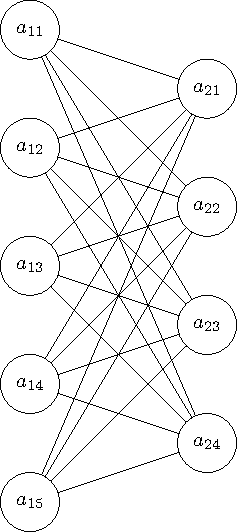
\includegraphics[height=0.6\textheight]{support/figures/neural.pdf}
        \end{figure}

        \note{绘制神经网络图像可能是非常适合 \TikZ{} 干的事情了,你说用 PowerPoint 繁琐的线段连接估计需要借助插件才能比较方便地实现。使用其他非编程性绘图工具都是比较头疼的事情。}
      }

      \only<2-3>{

        \pgf{} 提供 \cmd{foreach} 用来创建循环体,以绘制繁琐且结构类似的图。

        \vspace{4ex}

        \onslide<3>{
          \cmd{foreach} 可以嵌套使用。实际上 \cmd{foreach} 也可以接受多个参数的同时迭代,\cmd{foreach} \cmd{x}/\cmd{y} in \{1/2,2/3,3/4\} \{循环体\}。
        }
      }

      \only<4>{
        \TikZ{} 提供 \cmd{tikzstyle} 命令用于设定一个样式别称。\note{类似于 HTML 中的 class 然后通过 CSS 设定样式。}之后的节点或者边就可以直接套用该样式。

        \note{更多方法参见手册,内容非常多。}
      }

    \end{column}
    \begin{column}{0.6\textwidth}
      \begin{codeblock}[basicstyle=\ttfamily\scriptsize]{神经网络}
\documentclass[tikz]{standalone}
\begin{document}
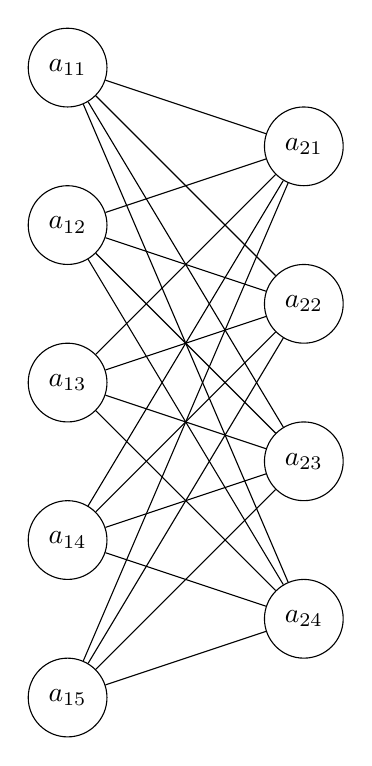
\begin{tikzpicture}
|\highlightline<4>|\tikzstyle{neuron}=[circle,draw,minimum width=1cm];
|\highlightline<2>|\foreach \x in {1,...,5} {
|\highlightline<4>|  \node[neuron] (a\x) at (0,-2*\x) {$a_{1\x}$};
}
\foreach \y in {1,...,4} {
|\highlightline<4>|  \node[neuron] (b\y) at (3,-1-2*\y) {$a_{2\y}$};
}
|\highlightline<3>|\foreach \x in {1,...,5} {
|\highlightline<3>|  \foreach \y in {1,...,4} {
    \draw (a\x) edge (b\y);
  }
}
\end{tikzpicture}
\end{document}
      \end{codeblock}
    \end{column}
  \end{columns}
\end{frame}

\begin{frame}[fragile]
  \frametitle{思维导图}
  \begin{columns}
    \begin{column}{0.4\textwidth}
      还可以通过 \cmd{usetikzlibrary} 调用内置库来绘制更多类型的图像。
      比如 \pkg{mindmap} 可以用来绘制思维导图 \link{https://mirrors.sjtug.sjtu.edu.cn/CTAN/graphics/pgf/base/doc/images/pgfmanual-mindmap-1.pdf}。

      \note{声明该 \env{tikzpicture} 为 \opt{mindmap} 类型,并使用 \opt{child} 指示子级,一个父级可以跟多个子级,子级可以嵌套子级。\opt{grow} 参数用来指示旋转角度,最后需要用分号结束。如果不想手动设定旋转角度,还可以在整幅图上使用 \opt{grow cyclic} 参数,如果想要实现这个链接所实现的效果,建议查看 \pgf{} 手册的 Tutorial 部分。}

      \begin{figure}
        \centering
        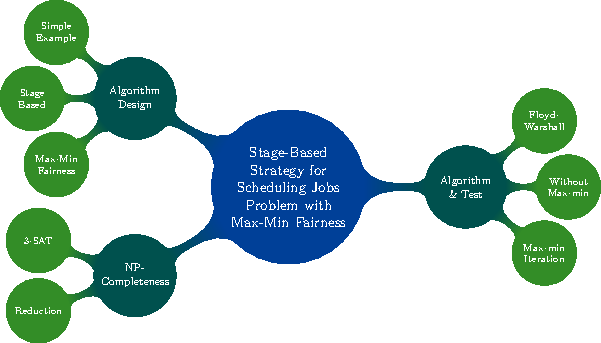
\includegraphics[height=0.35\textheight]{support/figures/mindmap.pdf}
        \caption{\ttfamily \pkg{mindmap} (tikzlibrary)}
      \end{figure}
    \end{column}
    \begin{column}{0.6\textwidth}
      \begin{codeblock}[]{\pkg{mindmap} 框架}
\documentclass[tikz]{standalone}
|\highlightline|\usetikzlibrary{mindmap}
\begin{document}
\begin{tikzpicture}[mindmap, concept color=blue]
\node [concept] {Parent} 
child [concept color=gray, grow=150] {
  node [concept] {Child1}}
child [concept color=gray, grow=0] {
  node [concept] {Child2}};
\end{tikzpicture}
\end{document}
      \end{codeblock}
    \end{column}
  \end{columns}

  \note{\pkg{mindmap} 库是 \TikZ{} 中非常 iconic 的一个库。文档中专门有一个例子来展示这个功能。}
\end{frame}

\begin{frame}
  \frametitle{\TikZ{}Edt}
  \includeinlinelogo{support/images/tikzedt.png} \TikZ{}Edt \link{http://www.tikzedt.org/} 是一款半图形化的即时绘图编辑器,在 \faWindows{} 上工作较好。

  \begin{columns}
    \begin{column}{0.4\textwidth}
      \begin{itemize}
        \item 善用工具栏功能 \link{http://www.tikzedt.org/doc.html}
        
        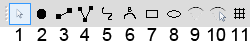
\includegraphics[width=\linewidth]{support/images/tooltip.png}
        \item 开始时会提示生成缩略图
        
        {\tiny Compilation $\blacktriangleright$ Compile snippet thumbnails}
        \item 如果有时编译不成功了,尝试重新预编译头
        
        {\tiny Compilation $\blacktriangleright$ (Re-)Generate precompiled headers}
        \item 可以更改头文件
        
        {\tiny Settings $\blacktriangleright$ Settings $\blacktriangleright$ Compiler}
      \end{itemize}
    \end{column}
    \begin{column}{0.6\textwidth}
      \begin{figure}
        \centering
        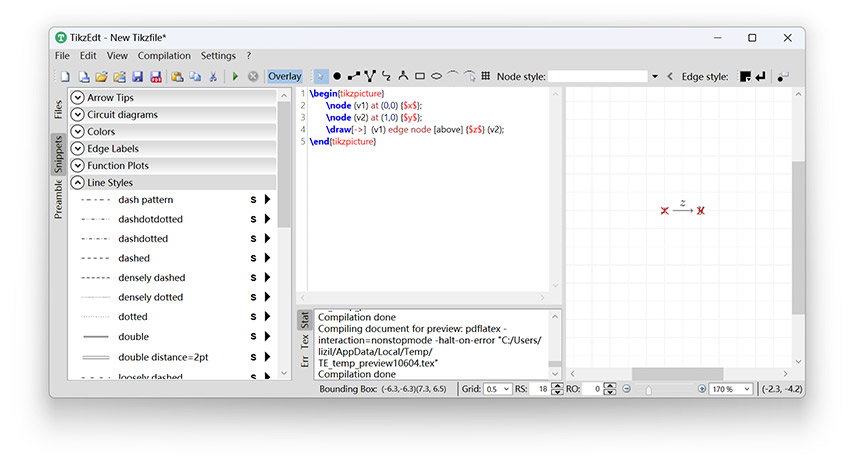
\includegraphics[height=0.5\textheight]{support/images/tikzedtui.jpg}
        \caption{\TikZ{}Edt 界面}
      \end{figure}
    \end{column}
  \end{columns}

  \note[item]{框架基于 Windows Presentation Foundation (WPF),代码开源于 Google Code。2014 年,该项目伴随着这个开源代码平台的终结也开发停止,作者跑路。其适配的 \faApple{} 版本由于跟不上 Mac OS 的更新似乎不再可用,在 \faLinux{} 上更趋向于一种模拟。本人希望在未来有空的时候将其从 .NET Framework 迁移到 .NET Core 上,修改一些脚本文件,以原生跨平台,主要看微软在迁移层面的表现(一般挺好)(本人也对 WPF 较为熟悉,但是这个框架也已慢慢地 deprecated,很多年前是比较流行的,主要这个是 \faWindows{} 专有框架)。}

  \note[item]{\faLinux{}\faApple{} 用户可能本身就更熟悉代码编写的方式,或者转向 Inkscape,以及希望 \TeX{}\textsc{macs} 越来越好(其自带的绘图编辑器看起来也很优秀),这样就可以直接所见即所得了。}
\end{frame}

\section{PGFPlots}

\begin{frame}[fragile]
  \frametitle{PGFPlots}
  \begin{columns}
    \begin{column}{0.4\textwidth}

      \only<1>{
        \pgfplots{} \link{https://mirrors.sjtug.sjtu.edu.cn/CTAN/graphics/pgf/contrib/pgfplots/doc/pgfplots.pdf} 是 \pgf{}/\TikZ{} 的衍生宏包,用于生成高质量中等数据规模的统计图。

        \begin{center}
          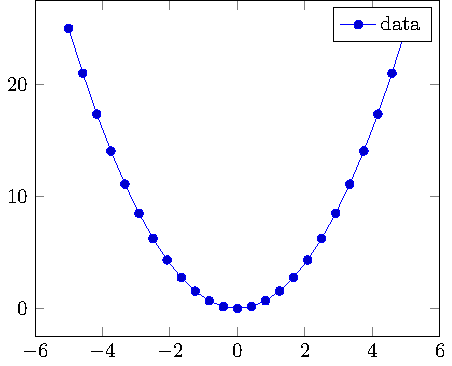
\includegraphics[width=0.75\textwidth]{support/figures/pgfplots.pdf}
        \end{center}
      }

      \only<2>{
        引入 \pgfplots{} 包,然后通过 \cmd{pgfplotsset} 设定版本和其他全局设定。
      }

      \only<3>{
        \env{axis} 环境用于插入 \pgfplots{} 统计图。
      }

      \only<4>{
        \cmd{addplot} 命令用于新建一个数据序列,其后不跟类型的情况下为关于 $x$ 的函数图像。

        \begin{table}
          \centering
          \footnotesize
          \begin{tabular}{>{\ttfamily}ll}
            \cmd{addplot} & 函数 \\
            \cmd{addplot} coordinates & 坐标点 \\
            \cmd{addplot} table & 文件表格 \\
          \end{tabular}
        \end{table}
      }

      \only<5>{
        \cmd{legend} 用于创建图例,使用逗号分隔每个序列的名称。
      }

    \end{column}
    \begin{column}{0.6\textwidth}
      
      \begin{codeblock}[]{使用 \pgfplots{}}
\documentclass[tikz]{standalone}
|\highlightline<2>|\usepackage{pgfplots}
|\highlightline<2>|\pgfplotsset{compat=newest}
\begin{document}
|\highlightline<3>|\begin{axis}
|\highlightline<4>|  \addplot {x^2};
|\highlightline<5>|  \legend{data,};
|\highlightline<3>|\end{axis}
|\phantom{}|\end{document}
      \end{codeblock}
      
    \end{column}
  \end{columns}
\end{frame}

\begin{frame}[fragile]
  \frametitle{PGFPlotsTable}

  \begin{columns}
    \begin{column}{0.4\textwidth}
      
      \only<1>{
        \pgfplotstable{} \link{https://mirrors.sjtug.sjtu.edu.cn/CTAN/graphics/pgf/contrib/pgfplots/doc/pgfplotstable.pdf} 是用于数据处理的子包,可以用来从文件排印表格。

        \begin{center}
          \includepdflarge{support/examples/pgfplotstable.pdf}
        \end{center}
      }

      \only<2>{
        \cmd{pgfplotstableset} 用于设定全局设置。这里设定了默认使用 CSV 文件,表格采用标准三线表格式。

        \begin{block}{\faInfo{}}
          SJTUBeamer 已经预先设置了这些格式。
        \end{block}
      }

      \only<3>{
        \cmd{pgfplotstabletypeset} 用于从文件排印表格。这样你的 CSV 文件就可以通过 Excel 软件编辑与处理。
        \note{又一层内容与格式分离!}

        \begin{block}{\faExclamationTriangle}
          含有中文内容的表格需要使用 \hologo{XeLaTeX} 编译!
        \end{block}
      }

    \end{column}
    \begin{column}{0.6\textwidth}
      
      \begin{codeblock}[]{使用 \pgfplotstable{}}
\documentclass{ctexart}
\usepackage{booktabs}
|\highlightline<1>|\usepackage{pgfplotstable}
\pgfplotsset{compat=newest}
|\highlightline<2>|\pgfplotstableset{
  col sep=comma,
  every head row/.style={before row=\toprule,after row=\midrule},
  every last row/.style={
    after row=\bottomrule},
}
\begin{document}
|\highlightline<3>|  \pgfplotstabletypeset[]{data.csv}
|\phantom{}|\end{document}
      \end{codeblock}
      
    \end{column}
  \end{columns}

\end{frame}

\begin{frame}
  \frametitle{PGFPlotsEdt}
  \includeinlinelogo{support/images/pgfplotsedt.pdf} PGFPlotsEdt \link{https://logcreative.github.io/PGFPlotsEdt/?lang=cn} 是一款基于 \pgfplots{} 的统计绘图编辑器,基于 \faVuejs{} 开发。

  \begin{columns}
    \begin{column}{0.4\textwidth}
      \begin{itemize}
        \item 顶部按钮提供了一些示例。
        \item 推荐首先在设定中设置好参数(比如三维)。
        \item 可以设置坐标系相关样式。
        \item 直接按下 \faExclamationTriangle{} 手动编辑代码。
        \note{按下没有回头路。因为回头路我没做好。}
      \end{itemize}
    \end{column}
    \begin{column}{0.6\textwidth}
      \begin{figure}
        \centering
        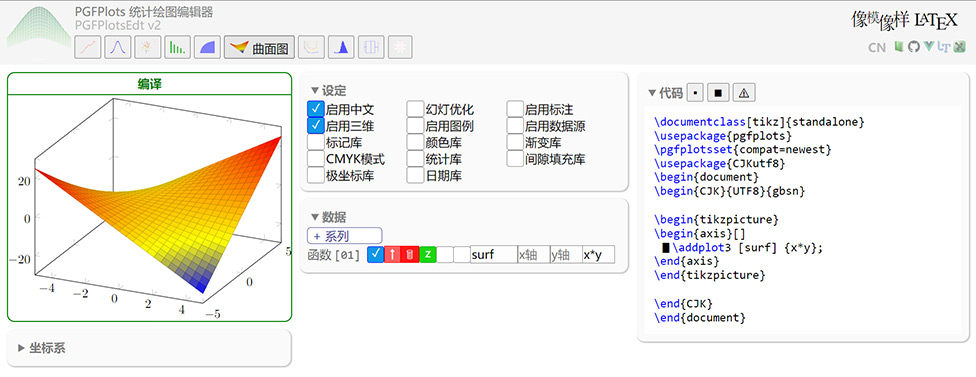
\includegraphics[height=0.4\textheight]{support/images/pgfplotsedtui.jpg}
        \caption{PGFPlotsEdt 界面}
      \end{figure}
    \end{column}
  \end{columns}

  \note{当年是想做个跟 \TikZ{}Edt 类似的软件,用于快速生成统计图代码。也想过使用 Qt 写,当然后面放弃了,转向编写网页应用。当时本人还没有什么服务器,就写了个纯前端。}

  \note{我为什么后来想翻译 Learn\LaTeX{}.org,也是因为我看到了它使用的编辑器框架与轻量级编译服务,非常适合用来开发小型软件,PGFPlotsEdt 也就是这个思想的实践。}
\end{frame}

\begin{frame}
  \frametitle{PGFPlotsEdt 帮助我完成物理实验报告图...}
  \begin{columns}
    \begin{column}{0.25\textwidth}
      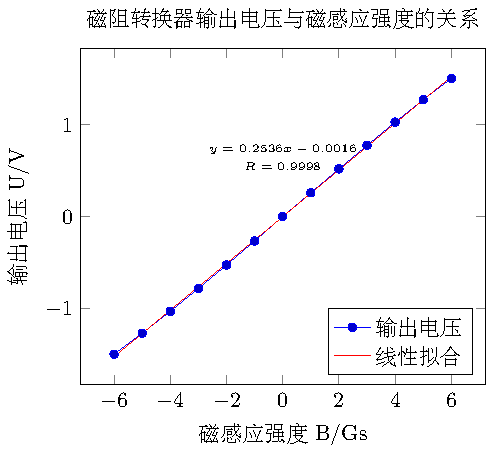
\includegraphics[width=\linewidth]{support/pgfplots/a.pdf}
      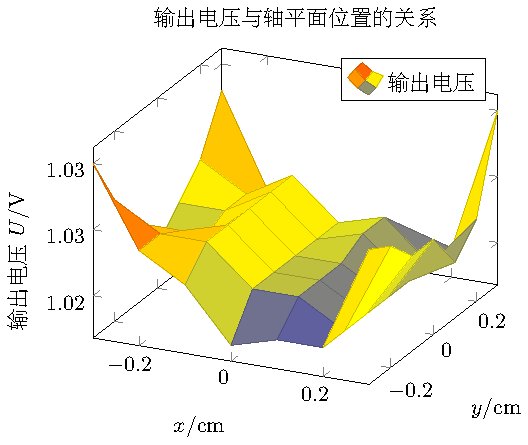
\includegraphics[width=\linewidth]{support/pgfplots/b.pdf}
    \end{column}
    \begin{column}{0.50\textwidth}
      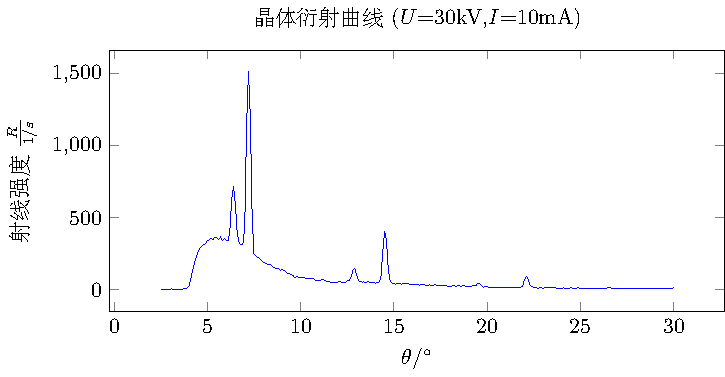
\includegraphics[width=\linewidth]{support/pgfplots/c.pdf}
      \begin{columns}
        \begin{column}{0.5\linewidth}
          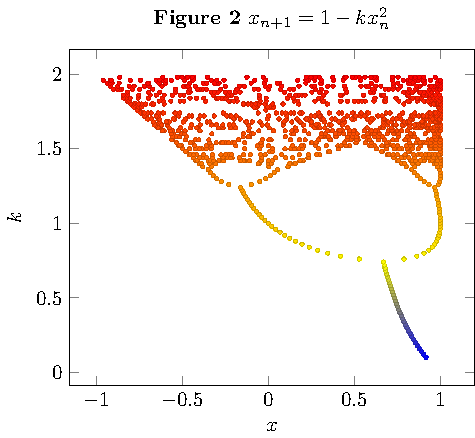
\includegraphics[width=\linewidth]{support/pgfplots/d.pdf}
        \end{column}
        \begin{column}{0.5\linewidth}
          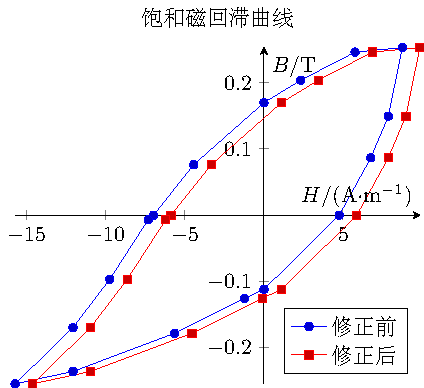
\includegraphics[width=\linewidth]{support/pgfplots/e.pdf}
        \end{column}
      \end{columns}
    \end{column}
    \begin{column}{0.25\textwidth}
      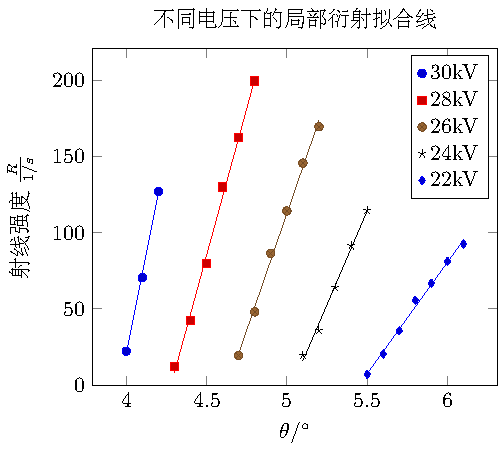
\includegraphics[width=\linewidth]{support/pgfplots/f.pdf}
      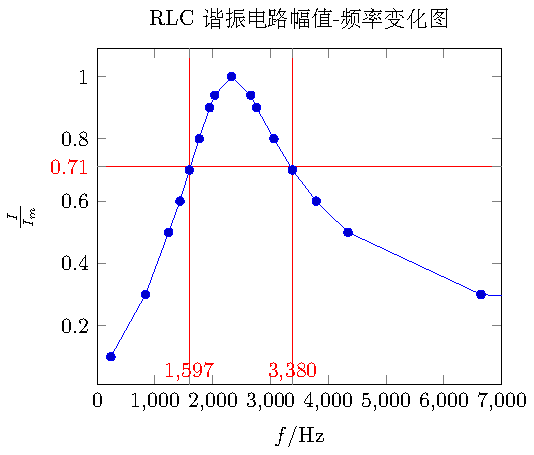
\includegraphics[width=\linewidth]{support/pgfplots/g.pdf}
    \end{column}
  \end{columns}
\end{frame}

\begin{frame}
  \frametitle{更多可能}

  \begin{columns}
    \begin{column}{0.58\textwidth}
      \begin{itemize}
        \item \TikZ{} 还内置很多的库可供使用!
        \item \TikZ{} 还有很多的衍生库可供使用!
        \note[item]{不只是 \pgfplots{}。}
        \item 推荐使用 \cls{standalone} 文档类编译再插入。
        \item 内存不足时需要使用 \hologo{LuaLaTeX} 编译。
        \note[item]{\hologo{LuaLaTeX} 使用了动态内存。之前的一个分形图就是因为需要大量的内存需要 \hologo{LuaLaTeX} 编译。}
        \item 使用 \pkg{external} 库缓存也是可行的。
        \item 更多内容请见手册\footnotemark。
      \end{itemize}
    \end{column}
    \begin{column}{0.42\textwidth}
      \begin{figure}
        \begin{tikzpicture}[scale=0.7,every node/.style={scale=0.7}]
          \node[draw,fill=white] (v1) at (-1.5,0) {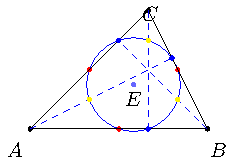
\includegraphics[scale=0.7]{support/figures/tkzeuclide.pdf}};
          \node[draw,fill=white] at (1.5,-2) {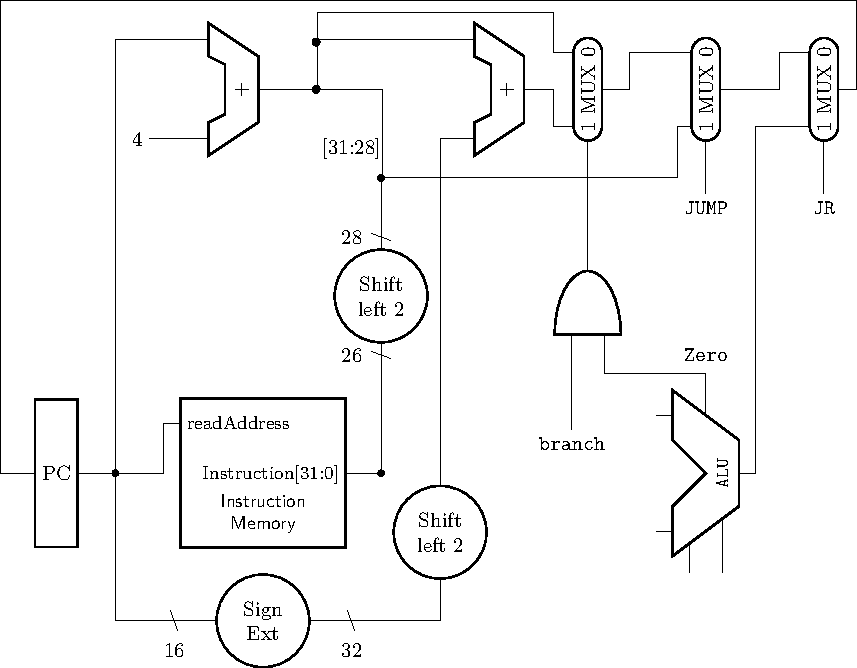
\includegraphics[scale=0.3]{support/figures/circuitikz.pdf}};
          \node[draw,fill=white] at (-1.5,-3) {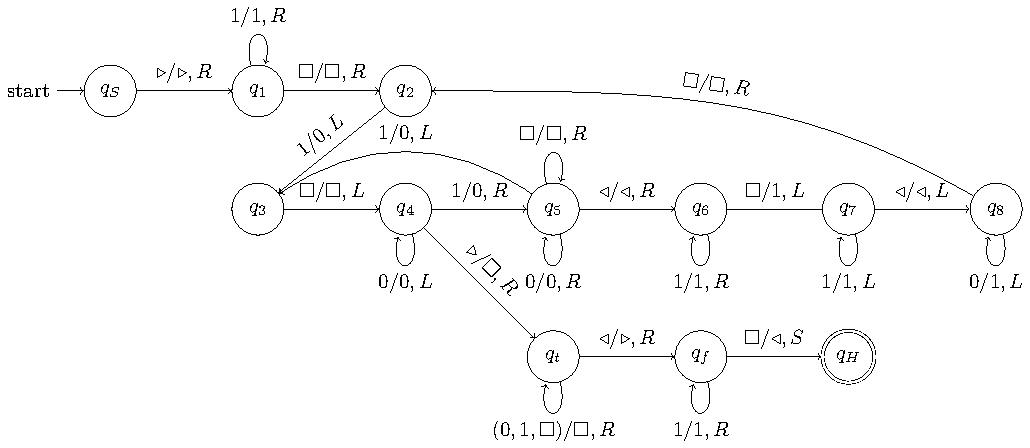
\includegraphics[scale=0.3]{support/figures/automata.pdf}};
        \end{tikzpicture}
        \caption{\ttfamily tkz-euclide \link{http://mirrors.sjtug.sjtu.edu.cn/CTAN/macros/latex/contrib/tkz/tkz-euclide/doc/tkz-euclide.pdf}, circuitikz \link{https://mirrors.sjtug.sjtu.edu.cn/CTAN/graphics/pgf/contrib/circuitikz/doc/circuitikzmanual.pdf}, automata (tikzlibrary)}
      \end{figure}
    \end{column}
  \end{columns}

  \footnotetext{(中文版)\LaTeX{} 工作室.
  \TikZ{} \& \pgf{} 手册 (3.1.5b) 笔记[EB/OL].
  2020. \link{https://www.latexstudio.net/archives/51804.html}}
  
  \note[item]{看文档需要使用 texdoc pgf,这个笔记大略翻译了很多内容。\LaTeX{} 工作室的网站上也有很多 \TikZ{} 的 fancy 内容,感兴趣的可以参考。}

  \note[item]{可以做的很 fancy,也可以用它很基本的功能。因为有一种职业叫科技绘图,这种图形约是符合要求的矢量图。\TikZ{} 的意义在于提供了一种 inline 绘图的方式,有助于管理工程,过早优化万恶之源,这样的方式有助于减少重新绘制的可能。}
  
\end{frame}
% !TeX root = ../../latex-talk.tex

\part{\LaTeX{} 无止境}

\begin{frame}
  \frametitle{宏包}

  \begin{itemize}
    \item 绝大多数 \LaTeX{} 宏包发布于 CTAN (Comprehensive \TeX{} Archive Network) \link{https://www.ctan.org/},1992 年建站以来,至今已经吸引 2855 名贡献者发布其 6215 个宏包。 
    \item \note{正如一般不会在简历上写精通 C 一样,也都}基本不敢写精通 \LaTeX{} \sout{(虽然没有什么大用}
    \item 可以通过编写宏来简化输入,可以阅读 \pkg{clsguide}\footnote{(中文版)刘海洋~译. 写给 \LaTeXe{} 类与宏包的作者[EB/OL]. 2010. \link{https://github.com/CTeX-org/ctex-doc/blob/master/clsguide-zh-cn/clsguide-zh-cn.tex}}, 
    \pkg{xparse}\footnote{(中文版)盛文博~译. \pkg{xparse} 宏包:进行文档命令解析[EB/OL]. 2018. \link{https://github.com/WenboSheng/LaTeX3-doc-cn/blob/master/xparse-doc-cn/xparse-cn.pdf}} 文档。
  \end{itemize}

  \begin{exampleblock}{定义宏举例}
    \begin{description}
      \item[\TeX] \cmd{def}\texttt{\textbackslash{}foo}\#1\#2\{\#1 of \#2\}
      \item[\LaTeXe] \cmd{newcommand}\texttt{\textbackslash{}foo}[2]\{\#1 of \#2\}
      \item[\LaTeX3] \cmd{NewDocumentCommand}\texttt{\textbackslash{}foo}\{mm\}\{\#1 of \#2\}
    \end{description}
  \end{exampleblock}

  \note{简单了解即可。}
  
\end{frame}

\begin{frame}[fragile]
  \frametitle{错误}
  \begin{columns}
    \begin{column}{0.55\textwidth}
      \begin{codeblock}[]{未定义命令}
\newcommand\mycommand{\textbold{hmmm}}
My command is used here \mycommand.
      \end{codeblock}
      \begin{codeblock}[]{括号不配对}
\usepackage[leqno}{amsmath}
      \end{codeblock}
    \end{column}
    \begin{column}{0.45\textwidth}
      \begin{codeblock}[]{文件缺失}
\usepackage{amsmathz}
      \end{codeblock}
      \begin{codeblock}[]{数学模式有空行}
\begin{equation}

  1=2

\end{equation}
      \end{codeblock}
    \end{column}
  \end{columns}
\end{frame}

\begin{frame}[fragile]
  \frametitle{错误}
  \begin{columns}
    \begin{column}{0.55\textwidth}
      \begin{block}{未定义命令}
        \begin{lstlisting}
! Undefined control sequence.
\mycommand ->\textbold 
                        {hmmm}
l.8 My command is used here \mycommand
                                      .
? 
        \end{lstlisting}
      \end{block}
      \begin{block}{括号不配对}
        \begin{lstlisting}
! Argument of \@fileswith@ptions has an extra }.
        \end{lstlisting}
      \end{block}
    \end{column}
    \begin{column}{0.45\textwidth}
      \begin{block}{文件缺失}
        \begin{lstlisting}
! LaTeX Error: File `amsmathz.sty' not found.
        \end{lstlisting}
        \note{检查是否安装了该宏包。或者宏包是否在搜索路径内。}
      \end{block}
      \begin{block}{数学模式有空行}
        \begin{lstlisting}
! Missing $ inserted.
        \end{lstlisting}
      \end{block}
    \end{column}
  \end{columns}
\end{frame}

\begin{frame}
  \frametitle{编译速度}
  \begin{columns}
    \begin{column}{0.5\textwidth}
      \begin{exampleblock}{\faWindows}
        \begin{itemize}
          \item \hologo{pdfLaTeX} 仍是目前最快的。
          \item 中文支持方面需要做变通方法。
          \item I/O 速度成为瓶颈。
        \end{itemize}
      \end{exampleblock}
    \end{column}
    \begin{column}{0.5\textwidth}
      \begin{exampleblock}{\faLinux{} \faApple}
        \begin{itemize}
          \item \hologo{XeLaTeX} 已经足够快。
          \item \CTeX{} 需要 \hologo{XeLaTeX} 或 \hologo{LuaLaTeX}。
          \item 主要取决于单核性能。
        \end{itemize}
      \end{exampleblock}
    \end{column}
  \end{columns}
  \begin{columns}
    \begin{column}{0.5\textwidth}
      \begin{block}{文章}
        \begin{itemize}
          \item \LaTeX{} 的主要设计用途。
          \item \hologo{pdfLaTeX}, \hologo{XeLaTeX} 和 \hologo{LuaLaTeX} 理想状态下速度差距不大 \link{https://stone-zeng.github.io/2019-07-24-tex-benchmark/}。
        \end{itemize}
      \end{block}
    \end{column}
    \begin{column}{0.5\textwidth}
      \begin{block}{幻灯}
        \begin{itemize}
          \item \LaTeX{} 的图形偏门流派。
          \item 由于 \textsc{pgf} 的引入使得 \hologo{LuaLaTeX} 明显偏慢。
        \end{itemize}
      \end{block}
    \end{column}
  \end{columns}

  \note[item]{魔兽争霸 3 当年出来的时候战役模式是主流,后来大家都开始打 RPG, DotA(没错,发源地),自定义的一些内容也可以很精彩。}

  \note[item]{用 PowerPoint 做完幻灯片会有一种空虚感,因为可能会做大量的重复工作。而 beamer 如果使用的好的话不会。}
\end{frame}

\begin{frame}
  \frametitle{加速轮子}
  \begin{columns}
    \begin{column}{0.33\textwidth}
      \begin{exampleblock}{ReportBoost \link{https://github.com/LogCreative/ReportBoost}}
        \begin{tabular}{p{0.9\textwidth}}
          提供一个已经配置完备的 Visual Studio Code 预编译工程目录。\\
          \midrule
          主要使用 \hologo{eTeX} 对 \hologo{pdfLaTeX} 在 \faWindows{} 上转储头文件为一个中间文件,减少 I/O 操作。
          \note{\hologo{eTeX} 是原生 \TeX{} 的扩展版本,支持更多的字符数,\hologo{XeTeX} 和 \hologo{LuaTeX} 基于其演变而来。}\\
          \midrule
          对 \hologo{XeLaTeX} 和 \hologo{LuaLaTeX} 支持不佳。
        \end{tabular}
      \end{exampleblock}
    \end{column}
    \begin{column}{0.33\textwidth}
      \begin{exampleblock}{AutoBeamer \link{https://github.com/LogCreative/AutoBeamer}}
        \begin{tabular}{p{0.9\textwidth}}
          主要提供将 \faMarkdown{} 文件翻译为 \LaTeX{} \cls{beamer} 代码的功能。\\
          \midrule
          \pkg{pandoc} \link{https://pandoc.org/index.html} 也可以将 \faMarkdown{} 转换为 \LaTeX{} 幻灯片代码,但结果不够干净。\\
          \midrule
          使用网页脚本语言 \faJs{} 造轮子主要考虑跨平台与未来功能迁移的可能。
        \end{tabular}
      \end{exampleblock}
    \end{column}
    \begin{column}{0.33\textwidth}
      \begin{exampleblock}{BeamerBoost \link{https://github.com/LogCreative/BeamerBoost}}
        \begin{tabular}{p{0.9\textwidth}}
          主要提供对 \cls{beamer} 文档类自然切割单位(帧)的脏区与并行渲染实现,更早拿到每帧结果。\\
          \midrule
          目前只能采用预编译的手段减少进程切换开销,主要面向 \faWindows{} 编译较慢情况的预览。\\
          \midrule
          导航栏结果未必准确。
        \end{tabular}
      \end{exampleblock}
    \end{column}
  \end{columns}

  \note{这些程序还都处于相互分离的阶段。但是也可以看到这种使用 Unix 哲学所涉及的程序带来的好处:每一个程序只做好一件事。模块化、尽可能使用文本输入输出流有助于程序的构建与修改,每一个部分都可以换成新的零件。}

  \note{beamer(与动画 \pkg{animate}) 可能是目前 \LaTeX{} 方面唯一有可能并行化的东西。}
\end{frame}


\def\bottomthanks{Happy \TeX{}ing!}
\makebottom